\section{张量范畴}

本章所论范畴默认是小的, 以免去一些不必要的集合论的困难.

\subsection{幺半范畴}

\subsubsection{定义}

\begin{example}
    我们先来考虑一类最简单的幺半范畴, 对于一个只有一个对象的严格 \(2\) - 范畴,
    定义一个范畴, 其对象为 \(\mathrm{Hom} (\bullet,\bullet)\), 态射为 \(2\) - 态射.

    注意到有择定对象 \(\mathbf{1} = \mathrm{id}\), 并且给出了 \(\mathrm{id} \circ -\) 和 \(- \circ \mathrm{id}\)
    作为范畴的自同构, 对于两个对象, 可以找到对应的 \(f \circ g\), 对于两个态射, 亦给出对应的合成为横合成.
\end{example}

\begin{definition}[幺半范畴]
    \label {definition:monoidal category}

    一个幺半范畴包含资料 \((\mathcal{C},\otimes,a,\mathbf{1},\iota)\), 其中 \(\mathcal{C}\) 是一个范畴,
    \(\otimes\) 是一个 \(\mathcal{C} \times \mathcal{C} \to \mathcal{C}\) 的函子, \(a\) 是两个 \(\mathcal{C} \times \mathcal{C} \times \mathcal{C} \to \mathcal{C}\)
    函子间的自然同构 \((- \otimes -) \otimes - \to - \otimes (- \otimes -)\) 称结合同构, \(\mathbf{1}\) 是 \(\mathcal{C}\) 中对象, 
    而 \(\iota\) 给出态射 \(\mathbf{1} \otimes \mathbf{1} \to \mathbf{1}\).

    满足五边形公理:
    \setlabel {五边形公理}
    \label {axiom:MC pentagon axiom}

    \begin{center}
        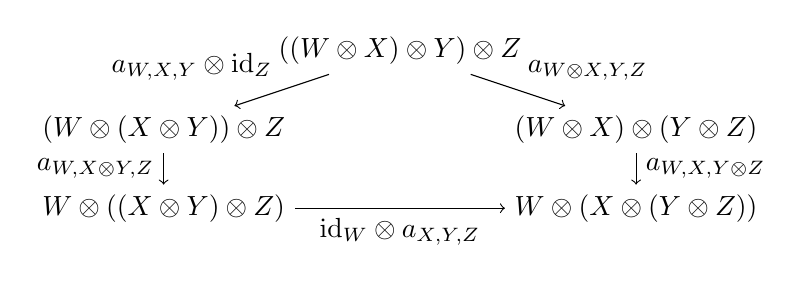
\begin{tikzpicture}
            \node (ararar) at (0,1) {\(((W \otimes X) \otimes Y) \otimes Z\)};
            \node (araarr) at (3,0) {\((W \otimes X) \otimes (Y \otimes Z)\)};
            \node (aarrar) at (-3,0) {\((W \otimes (X \otimes Y)) \otimes Z\)};
            \node (aaarrr) at (3,-1) {\(W \otimes (X \otimes (Y \otimes Z))\)};
            \node (aararr) at (-3,-1) {\(W \otimes ((X \otimes Y) \otimes Z)\)};

            \draw[->] (ararar) to node[above right] {\(a_{W \otimes X,Y,Z}\)} (araarr);
            \draw[->] (ararar) to node[above left] {\(a_{W,X,Y} \otimes \mathrm{id}_Z\)} (aarrar);
            \draw[->] (araarr) to node[right] {\(a_{W,X,Y \otimes Z}\)} (aaarrr);
            \draw[->] (aarrar) to node[left] {\(a_{W,X \otimes Y,Z}\)} (aararr);
            \draw[->] (aararr) to node[below] {\(\mathrm{id}_W \otimes a_{X,Y,Z}\)} (aaarrr);
        \end{tikzpicture}
    \end{center}

    与单位公理, 即以下定义的
    \setlabel {单位公理}
    \label {axiom:MC unit axiom}

        \[
            \begin{aligned}
                L_1 &: X \mapsto \mathbf{1} \otimes X, f \mapsto f \otimes \mathrm{id}_{\mathbf{1}} \\
                R_1 &: X \mapsto X \otimes \mathbf{1}, f \mapsto \mathrm{id}_{\mathbf{1}} \otimes f
            \end{aligned}
        \]

    \(L_1,R_1\) 给出了范畴 \(\mathcal{C} \to \mathcal{C}\) 的等价.
\end{definition}

我们常常用 \(\mathcal{C}\) 代指幺半范畴 \((\mathcal{C},\otimes,a,\mathbf{1},\iota)\).

\begin{definition}[子幺半范畴]
    对一个幺半范畴 \((\mathcal{C}, \otimes,a,\mathbf{1},\iota)\) 其子幺半范畴是指资料 \((\mathcal{D}, \otimes,a,\mathbf{1},\iota)\),
    满足 \(\mathcal{D}\) 是 \(\mathcal{C}\) 的子范畴, 且上述资料构成幺半范畴
\end{definition}

\begin{definition}[对偶幺半范畴]
    对一个幺半范畴 \((\mathcal{C}, \otimes,a,\mathbf{1},\iota)\), 其对偶幺半范畴为资料 \((\mathcal{C}^{\mathrm{op}}, \otimes^\mathrm{op}, a^\mathrm{op},\mathbf{1},\iota)\),
    满足 \(X \otimes^\mathrm{op} Y = Y \otimes X\) 与结合同构的变换 \(a_{X,Y,Z}^{\mathrm{op}} := a_{Z,Y,X}^{-1}\).
\end{definition}

\subsubsection{基本性质}

在幺半范畴中进行讨论, 常常运用添上 \(\mathbf{1}\) 并且使用 \(a,\iota\) 进行消去的技巧.

\begin{definition}
    定义自然同构 \(\lambda,\rho\) 

    \[
        \begin{aligned}
            \lambda_X &: \mathbf{1} \otimes X \to X \\
            \rho_X &: X \otimes \mathbf{1} \to X
        \end{aligned}
    \]

    为以下态射在 \(L_1,R_1\) 下的逆:

    \[
        \begin{aligned}
            \mathbf{1} \otimes (\mathbf{1} \otimes X) &\xrightarrow{a_{\mathbf{1},\mathbf{1},X}^{-1}} (\mathbf{1} \otimes \mathbf{1}) \otimes X \xrightarrow{\iota \otimes \mathrm{id}_X} \mathbf{1} \otimes X \\
            (X \otimes \mathbf{1}) \otimes \mathbf{1} &\xrightarrow{a_{X,\mathbf{1},\mathbf{1}}} X \otimes (\mathbf{1} \otimes \mathbf{1}) \xrightarrow{\mathrm{id}_X \otimes \iota} X \otimes \mathbf{1}
        \end{aligned}
    \]

    或者写成等式:

    \[
        \begin{aligned}
            \mathrm{id}_{\mathbf{1}} \otimes \lambda_X &= (\iota \otimes \mathrm{id}_X) \circ a_{\mathbf{1},\mathbf{1},X}^{-1}\\
            \rho_X \otimes \mathrm{id}_{\mathbf{1}} &= (\mathrm{id}_X \otimes \iota) \circ a_{X,\mathbf{1},\mathbf{1}}
        \end{aligned}
    \]

    自然性源于其为自然变换的复合.
\end{definition}

\begin{lemma}
    自然变换 \(\lambda,\rho\) 满足如下等式:

    \[
        \begin{aligned}
            \lambda_{\mathbf{1} \otimes X} &= \mathrm{id}_{\mathbf{1}} \otimes \lambda_X \\
            \rho_{X \otimes \mathbf{1}} &= \rho_X \otimes \mathrm{id}_{\mathbf{1}}
        \end{aligned}
    \]

    \begin{proof}
        基于 \(\lambda,\rho\) 为自然变换, 给出所有映射皆为同构的交换图表:

        \begin{center}
            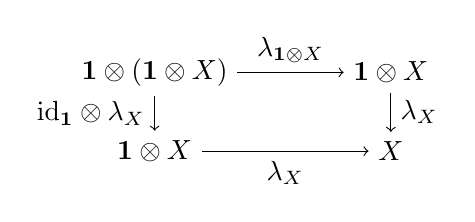
\begin{tikzpicture}
                \node (11x) at (-1.5,0.5) {\(\mathbf{1} \otimes (\mathbf{1} \otimes X)\)};
                \node (1x01) at (1.5,0.5) {\(\mathbf{1} \otimes X\)};
                \node (1x02) at (-1.5,-0.5) {\(\mathbf{1} \otimes X\)};
                \node (x) at (1.5,-0.5) {\(X\)};

                \draw[->] (11x) to node[above] {\(\lambda_{\mathbf{1} \otimes X}\)} (1x01);
                \draw[->] (11x) to node[left] {\(\mathrm{id}_{\mathbf{1}} \otimes \lambda_X\)} (1x02);
                \draw[->] (1x01) to node[right] {\(\lambda_X\)} (x);
                \draw[->] (1x02) to node[below] {\(\lambda_X\)} (x);
            \end{tikzpicture} 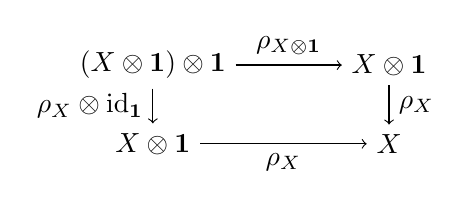
\begin{tikzpicture}
                \node (x11) at (-1.5,0.5) {\((X \otimes \mathbf{1}) \otimes \mathbf{1}\)};
                \node (x101) at (1.5,0.5) {\(X \otimes \mathbf{1}\)};
                \node (x102) at (-1.5,-0.5) {\(X \otimes \mathbf{1}\)};
                \node (x) at (1.5,-0.5) {\(X\)};

                \draw[->] (x11) to node[above] {\(\rho_{X \otimes \mathbf{1}}\)} (x101);
                \draw[->] (x11) to node[left] {\(\rho_X \otimes \mathrm{id}_{\mathbf{1}}\)} (x102);
                \draw[->] (x101) to node[right] {\(\rho_X\)} (x);
                \draw[->] (x102) to node[below] {\(\rho_X\)} (x);
            \end{tikzpicture}
        \end{center}
    \end{proof}
\end{lemma}

\begin{lemma}
    有交换图表:

    \begin{center}
        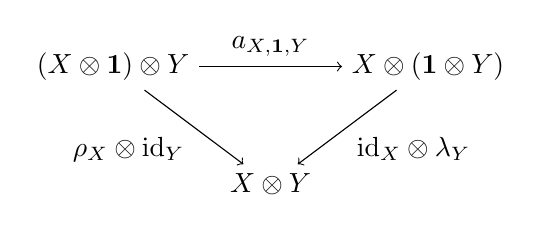
\begin{tikzpicture}
            \node (x1yl) at (-2,0.5) {\((X \otimes \mathbf{1}) \otimes Y\)};
            \node (x1yr) at (2,0.5) {\(X \otimes (\mathbf{1} \otimes Y)\)};
            \node (xy) at (0,-1) {\(X \otimes Y\)};

            \draw[->] (x1yl) to node[above] {\(a_{X,\mathbf{1},Y}\)} (x1yr);
            \draw[->] (x1yl) to node[below left] {\(\rho_X \otimes \mathrm{id}_Y\)} (xy);
            \draw[->] (x1yr) to node[below right] {\(\mathrm{id}_X \otimes \lambda_Y\)} (xy);
        \end{tikzpicture}
    \end{center}

    \begin{proof}
        注意到以下所有映射均为同构的交换图表, 其余小图形和外框交换, 故中心小三角形交换.

        \begin{center}
            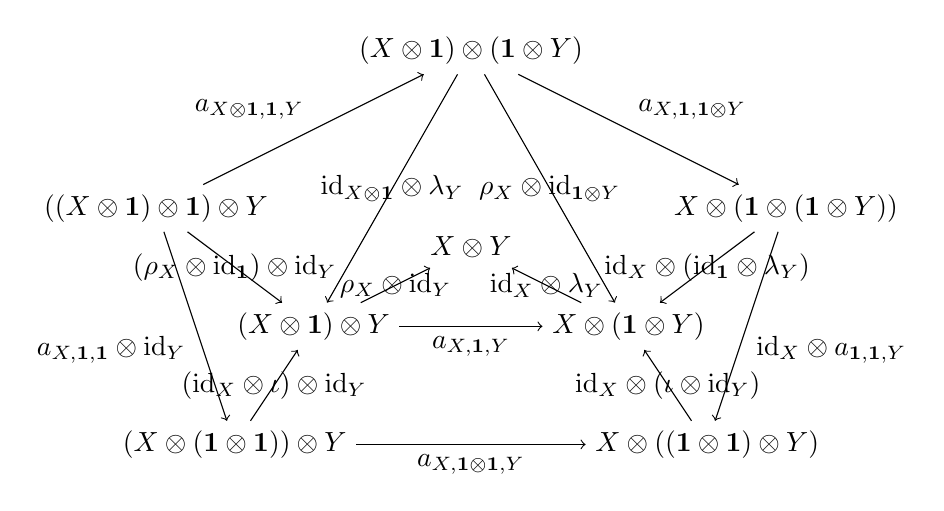
\begin{tikzpicture}
                \node (lx1rl1yr) at (0,3) {\((X \otimes \mathbf{1}) \otimes (\mathbf{1} \otimes Y)\)};
                \node (llx1r1ry) at (-4,1) {\(((X \otimes \mathbf{1}) \otimes \mathbf{1}) \otimes Y\)};
                \node (xl1l1yrr) at (4,1) {\(X \otimes (\mathbf{1} \otimes (\mathbf{1} \otimes Y))\)};
                \node (lxl11rry) at (-3,-2) {\((X \otimes (\mathbf{1} \otimes \mathbf{1})) \otimes Y\)};
                \node (xll11ryr) at (3,-2) {\(X \otimes ((\mathbf{1} \otimes \mathbf{1}) \otimes Y)\)};
                \node (lx1ry) at (-2,-0.5) {\((X \otimes \mathbf{1}) \otimes Y\)};
                \node (xl1yr) at (2,-0.5) {\(X \otimes (\mathbf{1} \otimes Y)\)};
                \node (xy) at (0,0.5) {\(X \otimes Y\)};

                \draw[->] (lx1rl1yr) to node[above right] {\(a_{X,\mathbf{1},\mathbf{1} \otimes Y}\)} (xl1l1yrr);
                \draw[->] (llx1r1ry) to node[above left] {\(a_{X \otimes \mathbf{1},\mathbf{1},Y}\)} (lx1rl1yr);
                \draw[->] (llx1r1ry) to node[below left] {\(a_{X,\mathbf{1},\mathbf{1}} \otimes \mathrm{id}_Y\)} (lxl11rry);
                \draw[->] (xl1l1yrr) to node[below right] {\(\mathrm{id}_X \otimes a_{\mathbf{1},\mathbf{1},Y}\)} (xll11ryr);
                \draw[->] (lxl11rry) to node[below] {\(a_{X,\mathbf{1} \otimes \mathbf{1},Y}\)} (xll11ryr);
                \draw[->] (lx1rl1yr) to node {\(\mathrm{id}_{X \otimes \mathbf{1}} \otimes \lambda_Y\)} (lx1ry);
                \draw[->] (lx1rl1yr) to node {\(\rho_X \otimes \mathrm{id}_{\mathbf{1} \otimes Y}\)} (xl1yr);
                \draw[->] (xl1l1yrr) to node {\(\mathrm{id}_X \otimes (\mathrm{id}_\mathbf{1} \otimes \lambda_Y)\)} (xl1yr);
                \draw[->] (xll11ryr) to node {\(\mathrm{id}_X \otimes (\iota \otimes \mathrm{id}_Y)\)} (xl1yr);
                \draw[->] (llx1r1ry) to node {\((\rho_X \otimes \mathrm{id}_\mathbf{1}) \otimes \mathrm{id}_Y\)} (lx1ry);
                \draw[->] (lxl11rry) to node {\((\mathrm{id}_X \otimes \iota) \otimes \mathrm{id}_Y\)} (lx1ry);
                \draw[->] (lx1ry) to node[below] {\(a_{X,\mathbf{1},Y}\)} (xl1yr);
                \draw[->] (lx1ry) to node {\(\rho_X \otimes \mathrm{id}_Y\)} (xy);
                \draw[->] (xl1yr) to node {\(\mathrm{id}_X \otimes \lambda_Y\)} (xy);
            \end{tikzpicture}
        \end{center}
    \end{proof}
\end{lemma}

\begin{corollary}
    上图中取 \(X = Y = \mathbf{1}\) 有:

    \[
        \lambda_{\mathbf{1}} = \rho_{\mathbf{1}} = \iota
    \]
\end{corollary}

\begin{lemma}
    有交换图表:

    \begin{center}
        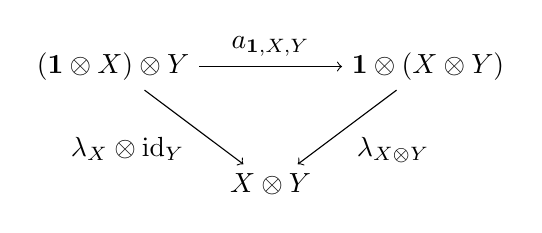
\begin{tikzpicture}
            \node (l1xry) at (-2,0.5) {\((\mathbf{1} \otimes X) \otimes Y\)};
            \node (1lxyr) at (2,0.5) {\(\mathbf{1} \otimes (X \otimes Y)\)};
            \node (xy) at (0,-1) {\(X \otimes Y\)};

            \draw[->] (l1xry) to node[above] {\(a_{\mathbf{1},X,Y}\)} (1lxyr);
            \draw[->] (l1xry) to node[below left] {\(\lambda_X \otimes \mathrm{id}_Y\)} (xy);
            \draw[->] (1lxyr) to node[below right] {\(\lambda_{X \otimes Y}\)} (xy);
        \end{tikzpicture}

        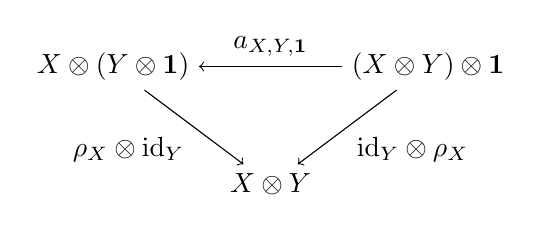
\begin{tikzpicture}
            \node (xly1r) at (-2,0.5) {\(X \otimes (Y \otimes \mathbf{1})\)};
            \node (lxyr1) at (2,0.5) {\((X \otimes Y) \otimes \mathbf{1}\)};
            \node (xy) at (0,-1) {\(X \otimes Y\)};

            \draw[->] (lxyr1) to node[above] {\(a_{X,Y,\mathbf{1}}\)} (xly1r);
            \draw[->] (lxyr1) to node[below right] {\(\mathrm{id}_Y \otimes \rho_X\)} (xy);
            \draw[->] (xly1r) to node[below left] {\(\rho_X \otimes \mathrm{id}_Y\)} (xy);
        \end{tikzpicture}
    \end{center}

    \begin{proof}
        同理观察全部态射均为同构的以下交换图表, 外框与其余小图形交换, 故左上角小三角形交换, 依赖 \(\mathbf{1} \otimes -\) 给出等价,
        第二幅图亦可对称的在对偶范畴中选取, 依赖 \(- \otimes \mathbf{1}\) 给出等价.

        \begin{center}
            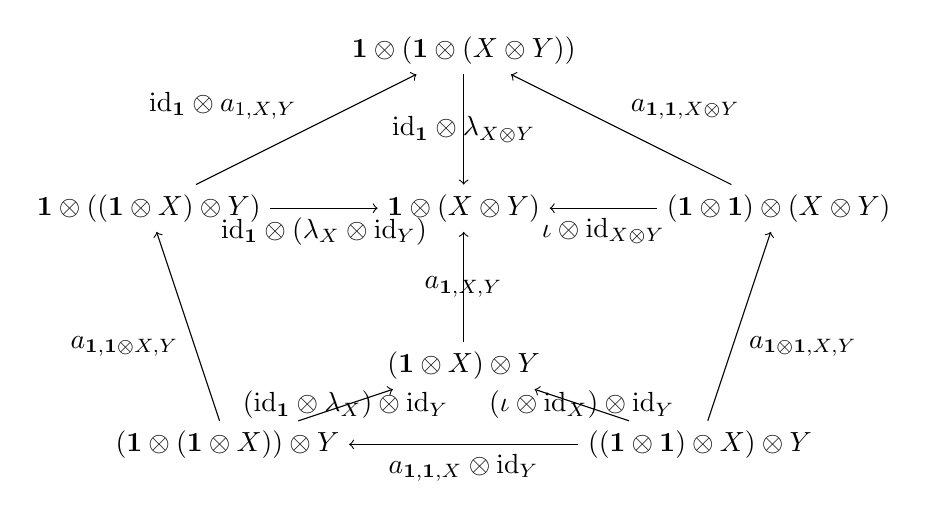
\begin{tikzpicture}
                \node (1ll1xryr) at (-4,1) {\(\mathbf{1} \otimes ((\mathbf{1} \otimes X) \otimes Y)\)};
                \node (l1l1xrry) at (-3,-2) {\((\mathbf{1} \otimes (\mathbf{1} \otimes X)) \otimes Y\)};
                \node (1l1lxyrr) at (0,3) {\(\mathbf{1} \otimes (\mathbf{1} \otimes (X \otimes Y))\)};
                \node (ll11rxry) at (3,-2) {\(((\mathbf{1} \otimes \mathbf{1}) \otimes X) \otimes Y\)};
                \node (l11rlxyr) at (4,1) {\((\mathbf{1} \otimes \mathbf{1}) \otimes (X \otimes Y)\)};
                \node (l1xry) at (0,-1) {\((\mathbf{1} \otimes X) \otimes Y\)};
                \node (1lxyr) at (0,1) {\(\mathbf{1} \otimes (X \otimes Y)\)};

                \draw[->] (1ll1xryr) to node[above left] {\(\mathrm{id}_\mathbf{1} \otimes a_{1,X,Y}\)} (1l1lxyrr);
                \draw[->] (l1l1xrry) to node[below left] {\(a_{\mathbf{1},\mathbf{1} \otimes X,Y}\)} (1ll1xryr);
                \draw[->] (ll11rxry) to node[below] {\(a_{\mathbf{1},\mathbf{1},X} \otimes \mathrm{id}_Y\)} (l1l1xrry);
                \draw[->] (l11rlxyr) to node[above right] {\(a_{\mathbf{1},\mathbf{1},X \otimes Y}\)} (1l1lxyrr);
                \draw[->] (ll11rxry) to node[below right] {\(a_{\mathbf{1} \otimes \mathbf{1},X,Y}\)} (l11rlxyr);
                \draw[->] (1ll1xryr) to node[below] {\(\mathrm{id}_\mathbf{1} \otimes (\lambda_{X} \otimes \mathrm{id}_Y)\)} (1lxyr);
                \draw[->] (l1l1xrry) to node {\((\mathrm{id}_\mathbf{1} \otimes \lambda_X) \otimes \mathrm{id}_Y\)} (l1xry);
                \draw[->] (1l1lxyrr) to node {\(\mathrm{id}_\mathbf{1} \otimes \lambda_{X \otimes Y}\)} (1lxyr);
                \draw[->] (ll11rxry) to node {\((\iota \otimes \mathrm{id}_X) \otimes \mathrm{id}_Y\)} (l1xry);
                \draw[->] (l11rlxyr) to node[below] {\(\iota \otimes \mathrm{id}_{X \otimes Y}\)} (1lxyr);
                \draw[->] (l1xry) to node {\(a_{\mathbf{1},X,Y}\)} (1lxyr);
            \end{tikzpicture}
        \end{center}
    \end{proof}
\end{lemma}

\begin{axiom}
    \setlabel {三角形公理}
    \label {axiom:MC triangle axiom}
    上述三个三角形交换图表称为三角形公理.
\end{axiom}

\begin{definition}[幺半范畴]
    一个幺半范畴包含资料 \((\mathcal{C},\otimes,a,\mathbf{1},\lambda,\rho)\), 其中 \(\mathcal{C}\) 是一个范畴,
    \(\otimes\) 是一个 \(\mathcal{C} \times \mathcal{C} \to \mathcal{C}\) 的函子, \(a\) 是两个 \(\mathcal{C} \times \mathcal{C} \times \mathcal{C} \to \mathcal{C}\) 函子间的自然同构,
    \(\mathbf{1}\) 是 \(\mathcal{C}\) 中对象, \(\lambda,\rho\) 是 \(\mathbf{1} \otimes -, - \otimes \mathbf{1} \to -\) 的自然同构, 满足 \ref{axiom:MC pentagon axiom}, \ref{axiom:MC triangle axiom}.

    \begin{proof}
        只需验证 \(\lambda_\mathbf{1} = \rho_\mathbf{1} = \iota\), 以及此给出的 \(\iota\) 诱导出同样的 \(\lambda,\rho\).

        反过来, 有下述图表交换, 于是最下方梯形交换, 从而 \(\lambda_\mathbf{1} = \rho_\mathbf{1} = \iota\), 
        \(\iota\) 给出 \(\lambda,\rho\) 是三角形公理取 \(X = \mathbf{1}\) 或 \(Y = \mathbf{1}\) 给出的.

        \begin{center}
            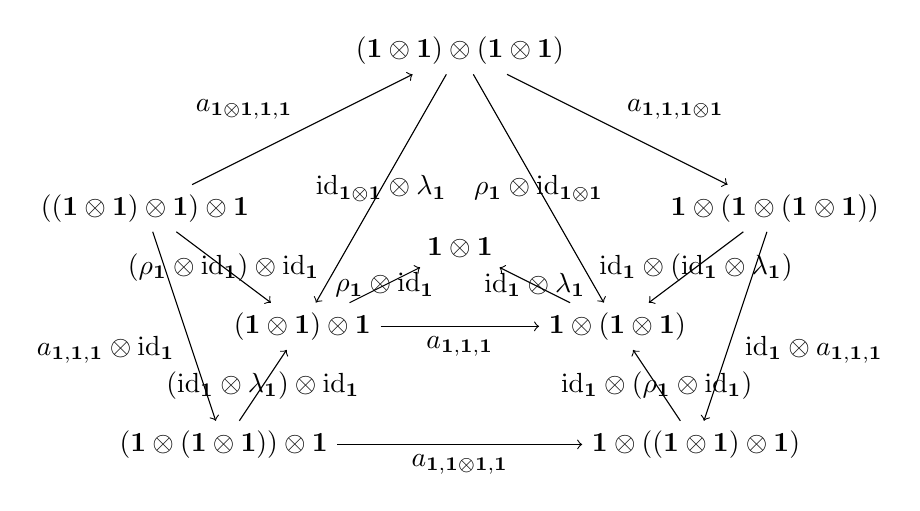
\begin{tikzpicture}
                \node (lx1rl1yr) at (0,3) {\((\mathbf{1} \otimes \mathbf{1}) \otimes (\mathbf{1} \otimes \mathbf{1})\)};
                \node (llx1r1ry) at (-4,1) {\(((\mathbf{1} \otimes \mathbf{1}) \otimes \mathbf{1}) \otimes \mathbf{1}\)};
                \node (xl1l1yrr) at (4,1) {\(\mathbf{1} \otimes (\mathbf{1} \otimes (\mathbf{1} \otimes \mathbf{1}))\)};
                \node (lxl11rry) at (-3,-2) {\((\mathbf{1} \otimes (\mathbf{1} \otimes \mathbf{1})) \otimes \mathbf{1}\)};
                \node (xll11ryr) at (3,-2) {\(\mathbf{1} \otimes ((\mathbf{1} \otimes \mathbf{1}) \otimes \mathbf{1})\)};
                \node (lx1ry) at (-2,-0.5) {\((\mathbf{1} \otimes \mathbf{1}) \otimes \mathbf{1}\)};
                \node (xl1yr) at (2,-0.5) {\(\mathbf{1} \otimes (\mathbf{1} \otimes \mathbf{1})\)};
                \node (xy) at (0,0.5) {\(\mathbf{1} \otimes \mathbf{1}\)};

                \draw[->] (lx1rl1yr) to node[above right] {\(a_{\mathbf{1},\mathbf{1},\mathbf{1} \otimes \mathbf{1}}\)} (xl1l1yrr);
                \draw[->] (llx1r1ry) to node[above left] {\(a_{\mathbf{1} \otimes \mathbf{1},\mathbf{1},\mathbf{1}}\)} (lx1rl1yr);
                \draw[->] (llx1r1ry) to node[below left] {\(a_{\mathbf{1},\mathbf{1},\mathbf{1}} \otimes \mathrm{id}_\mathbf{1}\)} (lxl11rry);
                \draw[->] (xl1l1yrr) to node[below right] {\(\mathrm{id}_\mathbf{1} \otimes a_{\mathbf{1},\mathbf{1},\mathbf{1}}\)} (xll11ryr);
                \draw[->] (lxl11rry) to node[below] {\(a_{\mathbf{1},\mathbf{1} \otimes \mathbf{1},\mathbf{1}}\)} (xll11ryr);
                \draw[->] (lx1rl1yr) to node {\(\mathrm{id}_{\mathbf{1} \otimes \mathbf{1}} \otimes \lambda_\mathbf{1}\)} (lx1ry);
                \draw[->] (lx1rl1yr) to node {\(\rho_\mathbf{1} \otimes \mathrm{id}_{\mathbf{1} \otimes \mathbf{1}}\)} (xl1yr);
                \draw[->] (xl1l1yrr) to node {\(\mathrm{id}_\mathbf{1} \otimes (\mathrm{id}_\mathbf{1} \otimes \lambda_\mathbf{1})\)} (xl1yr);
                \draw[->] (xll11ryr) to node {\(\mathrm{id}_\mathbf{1} \otimes (\rho_\mathbf{1} \otimes \mathrm{id}_\mathbf{1})\)} (xl1yr);
                \draw[->] (llx1r1ry) to node {\((\rho_\mathbf{1} \otimes \mathrm{id}_\mathbf{1}) \otimes \mathrm{id}_\mathbf{1}\)} (lx1ry);
                \draw[->] (lxl11rry) to node {\((\mathrm{id}_\mathbf{1} \otimes \lambda_\mathbf{1}) \otimes \mathrm{id}_\mathbf{1}\)} (lx1ry);
                \draw[->] (lx1ry) to node[below] {\(a_{\mathbf{1},\mathbf{1},\mathbf{1}}\)} (xl1yr);
                \draw[->] (lx1ry) to node {\(\rho_\mathbf{1} \otimes \mathrm{id}_\mathbf{1}\)} (xy);
                \draw[->] (xl1yr) to node {\(\mathrm{id}_\mathbf{1} \otimes \lambda_\mathbf{1}\)} (xy);
            \end{tikzpicture}
        \end{center}
    \end{proof}
\end{definition}

\subsubsection{幺半函子}

\begin{definition}[幺半函子]
    两个幺半范畴 \(\mathfrak{C} := (\mathcal{C},\otimes,a,\mathbf{1},\iota), \mathfrak{C}^\prime := (\mathcal{C}^\prime,\otimes^\prime,a^\prime,\mathbf{1}^\prime,\iota^\prime)\),
    一个幺半函子 \(\mathfrak{F} : \mathfrak{C} \to \mathfrak{C}^\prime\) 是一个函子 \(F : \mathcal{C} \to \mathcal{C}^\prime\), 与一个 \(\mathcal{C} \times \mathcal{C} \to \mathcal{C}^\prime\)
    上的自然同构 \(J :(F(-) \otimes^\prime F(-)) \to F ((-) \otimes (-))\), 与同构 \(F (\mathbf{1}) \to \mathbf{1}^\prime\), 以及以下交换图表:

    \begin{center}
        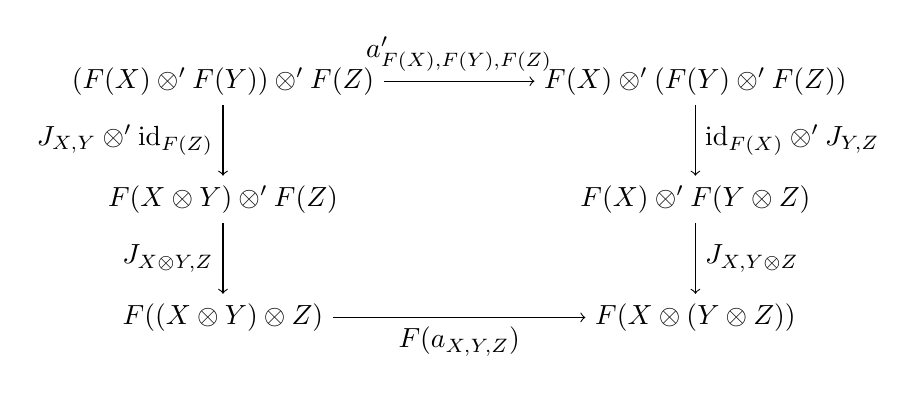
\begin{tikzpicture}
            \node (lfxfyrfz) at (-3,1.5) {\((F(X) \otimes^\prime F(Y)) \otimes^\prime F(Z)\)};
            \node (fxlfyfzr) at (3,1.5) {\(F(X) \otimes^\prime (F(Y) \otimes^\prime F(Z))\)};
            \node (fxyfz) at (-3,0) {\(F(X \otimes Y) \otimes^\prime F(Z)\)};
            \node (fxfyz) at (3,0) {\(F(X) \otimes^\prime F(Y \otimes Z)\)};
            \node (flxyrz) at (-3,-1.5) {\(F((X \otimes Y) \otimes Z)\)};
            \node (lfxlyzr) at (3,-1.5) {\(F(X \otimes (Y \otimes Z))\)};

            \draw[->] (lfxfyrfz) to node[above] {\(a^\prime_{F(X),F(Y),F(Z)}\)} (fxlfyfzr);
            \draw[->] (lfxfyrfz) to node[left] {\(J_{X,Y} \otimes^\prime \mathrm{id}_{F(Z)}\)} (fxyfz);
            \draw[->] (fxlfyfzr) to node[right] {\(\mathrm{id}_{F(X)} \otimes^\prime J_{Y,Z}\)} (fxfyz);
            \draw[->] (fxyfz) to node[left] {\(J_{X \otimes Y,Z}\)} (flxyrz);
            \draw[->] (fxfyz) to node[right] {\(J_{X,Y \otimes Z}\)} (lfxlyzr);
            \draw[->] (flxyrz) to node[below] {\(F(a_{X,Y,Z})\)} (lfxlyzr);
        \end{tikzpicture}
    \end{center}

    \setlabel {幺半结构公理}
    \label {axiom:MC monoidal functor axiom}
    以上图表称为幺半结构公理.
\end{definition}

\begin{definition}[幺半等价]
    一个幺半函子 \(\mathfrak{F} : \mathfrak{C} \to \mathfrak{C}^\prime\) 是一个幺半等价, 若 \(F\) 是 \(\mathcal{C} \to \mathcal{C}^\prime\) 的等价.
\end{definition}

\begin{lemma}
    \label {lemma:MC canonical isomorphism}
    同构 \(\phi : \mathbf{1}^\prime \to F(\mathbf{1})\) 有典范的选取, 使得以下所有映射皆为同构的交换图表成立:
    \begin{center}
        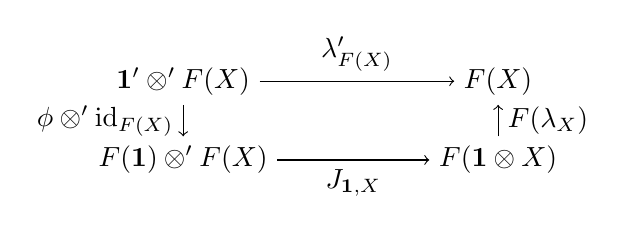
\begin{tikzpicture}
            \node (1fx) at (-2,0.5) {\(\mathbf{1}^\prime \otimes^\prime F(X)\)};
            \node (fx) at (2,0.5) {\(F(X)\)};
            \node (f1fx) at (-2,-0.5) {\(F(\mathbf{1}) \otimes^\prime F(X)\)};
            \node (f1x) at (2,-0.5) {\(F(\mathbf{1} \otimes X)\)};

            \draw[->] (1fx) to node[above] {\(\lambda^\prime_{F(X)}\)} (fx);
            \draw[->] (1fx) to node[left] {\(\phi \otimes^\prime \mathrm{id}_{F(X)}\)} (f1fx);
            \draw[->] (f1x) to node[right] {\(F(\lambda_X)\)} (fx);
            \draw[->] (f1fx) to node[below] {\(J_{\mathbf{1},X}\)} (f1x);
        \end{tikzpicture}
    \end{center}

    \begin{center}
        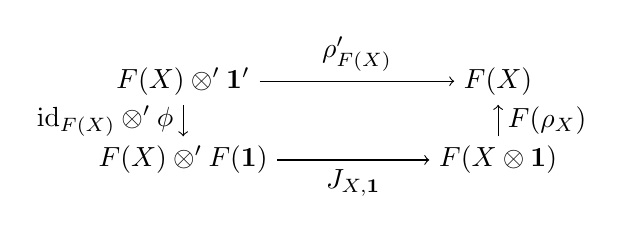
\begin{tikzpicture}
            \node (flxr1) at (-2,0.5) {\(F(X) \otimes^\prime \mathbf{1}^\prime\)};
            \node (fx) at (2,0.5) {\(F(X)\)};
            \node (fxf1) at (-2,-0.5) {\(F(X) \otimes^\prime F(\mathbf{1})\)};
            \node (flx1r) at (2,-0.5) {\(F(X \otimes \mathbf{1})\)};

            \draw[->] (flxr1) to node[above] {\(\rho^\prime_{F(X)}\)} (fx);
            \draw[->] (flxr1) to node[left] {\(\mathrm{id}_{F(X)} \otimes^\prime \phi\)} (fxf1);
            \draw[->] (flx1r) to node[right] {\(F(\rho_X)\)} (fx);
            \draw[->] (fxf1) to node[below] {\(J_{X,\mathbf{1}}\)} (flx1r);
        \end{tikzpicture}
    \end{center}

    \begin{proof}
        在第一幅图中取 \(X = \mathbf{1}\), 构造出对应的 \(\phi\), 函子 \(- \otimes^\prime F(\mathbf{1})\) 典范同构于函子 \(- \otimes^\prime \mathbf{1}^\prime\), 故其存在,
        需证明以上图表对于任意 \(X\) 成立.

        验证以下交换图表, 其余小图形与外框交换故左上大三角交换, 而依赖于 \(- \otimes^\prime F(\mathbf{1})\) 给出范畴等价知其给出第二幅图片, 在第二幅图中取 \(X = \mathbf{1}\)
        反过来可对称的验证第一幅图.

        \begin{center}
            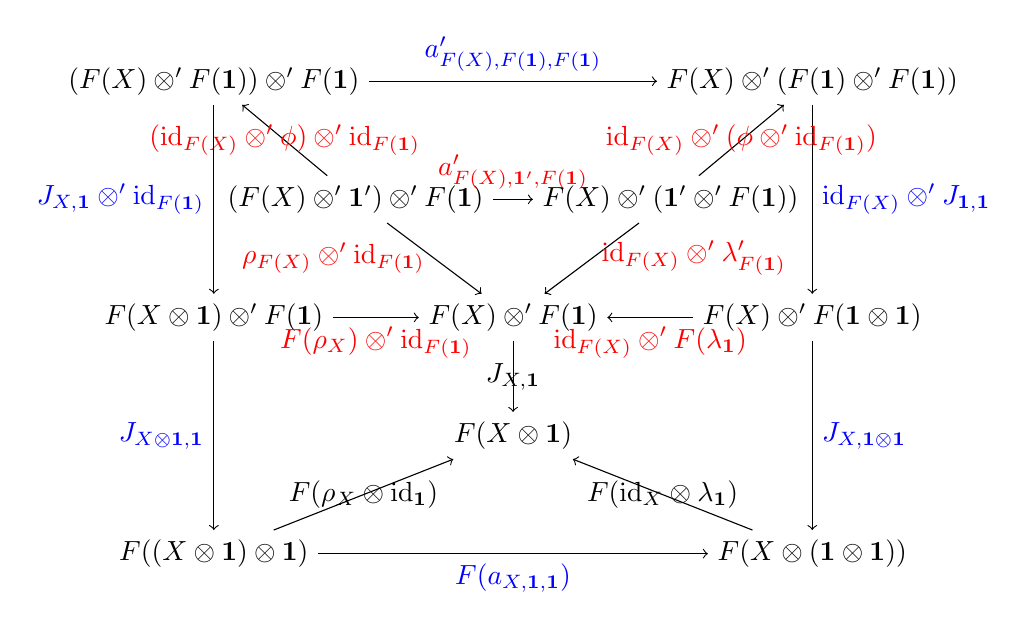
\begin{tikzpicture}
                \node (lfxf1rf1) at (-3.8,3) {\((F(X) \otimes^\prime F(\mathbf{1})) \otimes^\prime F(\mathbf{1})\)};
                \node (fxlf1f1r) at (3.8,3) {\(F(X) \otimes^\prime (F(\mathbf{1}) \otimes^\prime F(\mathbf{1}))\)};
                \node (lfx1rf1) at (-2,1.5) {\((F(X) \otimes^\prime \mathbf{1}^\prime) \otimes^\prime F(\mathbf{1})\)};
                \node (fxl1f1r) at (2,1.5) {\(F(X) \otimes^\prime (\mathbf{1}^\prime \otimes^\prime F(\mathbf{1}))\)};
                \node (fx1f1) at (-3.8,0) {\(F(X \otimes \mathbf{1}) \otimes^\prime F(\mathbf{1})\)};
                \node (fxf1) at (0,0) {\(F(X) \otimes^\prime F(\mathbf{1})\)};
                \node (fxf11) at (3.8,0) {\(F(X) \otimes^\prime F(\mathbf{1} \otimes \mathbf{1})\)};
                \node (fx1) at (0,-1.5) {\(F(X \otimes \mathbf{1})\)};
                \node (flx1r1) at (-3.8,-3) {\(F((X \otimes \mathbf{1}) \otimes \mathbf{1})\)};
                \node (fxl11r) at (3.8,-3) {\(F(X \otimes (\mathbf{1} \otimes \mathbf{1}))\)};

                \draw[->] (lfxf1rf1) to node[above] {\textcolor{blue}{\(a^\prime_{F(X),F(\mathbf{1}),F(\mathbf{1})}\)}} (fxlf1f1r);
                \draw[->] (lfx1rf1) to node {\textcolor{red}{\((\mathrm{id}_{F(X)} \otimes^\prime \phi) \otimes^\prime \mathrm{id}_{F(\mathbf{1})}\)}} (lfxf1rf1);
                \draw[->] (lfxf1rf1) to node[left] {\textcolor{blue}{\(J_{X,\mathbf{1}} \otimes^\prime \mathrm{id}_{F(\mathbf{1})}\)}} (fx1f1);
                \draw[->] (fxlf1f1r) to node[right] {\textcolor{blue}{\(\mathrm{id}_{F(X)} \otimes^\prime J_{\mathbf{1},\mathbf{1}}\)}} (fxf11);
                \draw[->] (lfx1rf1) to node[above] {\textcolor{red}{\(a^\prime_{F(X),\mathbf{1}^\prime,F(\mathbf{1})}\)}} (fxl1f1r);
                \draw[->] (fxl1f1r) to node {\textcolor{red}{\(\mathrm{id}_{F(X)} \otimes^\prime (\phi \otimes^\prime \mathrm{id}_{F(\mathbf{1})})\)}} (fxlf1f1r);
                \draw[->] (lfx1rf1) to node[left] {\textcolor{red}{\(\rho_{F(X)} \otimes^\prime \mathrm{id}_{F(\mathbf{1})}\)}} (fxf1);
                \draw[->] (fxl1f1r) to node[right] {\textcolor{red}{\(\mathrm{id}_{F(X)} \otimes^\prime \lambda^\prime_{F(\mathbf{1})}\)}} (fxf1);
                \draw[->] (fxf1) to node {\(J_{X,\mathbf{1}}\)} (fx1);
                \draw[->] (fx1f1) to node[below] {\textcolor{red}{\(F(\rho_X) \otimes^\prime \mathrm{id}_{F(\mathbf{1})}\)}} (fxf1);
                \draw[->] (fxf11) to node[below] {\textcolor{red}{\(\mathrm{id}_{F(X)} \otimes^\prime F(\lambda_\mathbf{1})\)}} (fxf1);
                \draw[->] (fx1f1) to node[left] {\textcolor{blue}{\(J_{X \otimes \mathbf{1},\mathbf{1}}\)}} (flx1r1);
                \draw[->] (fxf11) to node[right] {\textcolor{blue}{\(J_{X,\mathbf{1} \otimes \mathbf{1}}\)}} (fxl11r);
                \draw[->] (flx1r1) to node[below] {\textcolor{blue}{\(F(a_{X,\mathbf{1},\mathbf{1}})\)}} (fxl11r);
                \draw[->] (flx1r1) to node {\(F(\rho_X \otimes \mathrm{id}_\mathbf{1})\)} (fx1);
                \draw[->] (fxl11r) to node {\(F(\mathrm{id}_X \otimes \lambda_\mathbf{1})\)} (fx1);
            \end{tikzpicture}
        \end{center}
    \end{proof}
\end{lemma}

\begin{definition}[幺半函子]
    一个幺半函子是资料 \((F,J,\phi)\), 其中 \(F : \mathcal{C} \to \mathcal{C}^\prime\) 是一个函子, 
    \(J\) 是一个 \(\mathcal{C} \times \mathcal{C} \to \mathcal{C}^\prime\) 上的自然同构,
    \(\phi : \mathbf{1}^\prime \to F(\mathbf{1})\) 是一个同构, 满足 \ref{axiom:MC monoidal functor axiom} 与 \ref{lemma:MC canonical isomorphism} 中的图表.
\end{definition}

\begin{corollary}
    幺半函子的复合是幺半函子.

    \begin{proof}
        \(J^G\) 自然性可以给出交换图表, 将其嵌入定义与 \ref{axiom:MC monoidal functor axiom} 中的图表, 便得到复合幺半函子的幺半结构公理.

        \begin{center}
            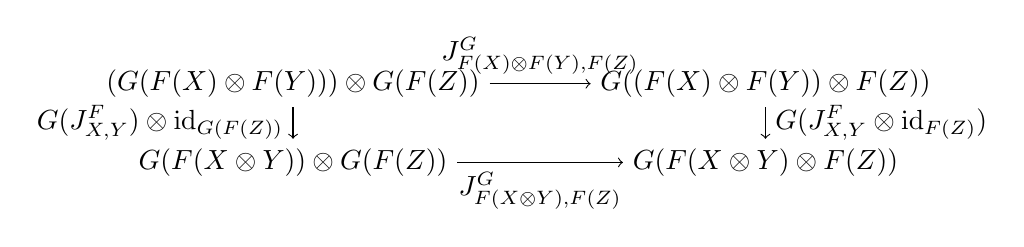
\begin{tikzpicture}
                \node (gfxfygfz) at (-3,0.5) {\((G(F(X) \otimes F(Y))) \otimes G(F(Z))\)};
                \node (gfxfyfz) at (3,0.5) {\(G((F(X) \otimes F(Y)) \otimes F(Z))\)};
                \node (gfxygfz) at (-3,-0.5) {\(G(F(X \otimes Y)) \otimes G(F(Z))\)};
                \node (gfxyfz) at (3,-0.5) {\(G(F(X \otimes Y) \otimes F(Z))\)};

                \draw[->] (gfxfygfz) to node[above] {\(J^G_{F(X) \otimes F(Y),F(Z)}\)} (gfxfyfz);
                \draw[->] (gfxfygfz) to node[left] {\(G(J^F_{X,Y}) \otimes \mathrm{id}_{G(F(Z))}\)} (gfxygfz);
                \draw[->] (gfxfyfz) to node[right] {\(G(J^F_{X,Y} \otimes \mathrm{id}_{F(Z)})\)} (gfxyfz);
                \draw[->] (gfxygfz) to node[below] {\(J^G_{F(X \otimes Y),F(Z)}\)} (gfxyfz);
            \end{tikzpicture}
        \end{center}
    \end{proof}
\end{corollary}

\begin{definition}
    两个幺半函子 \(F_1,F_2 : \mathfrak{C} \to \mathfrak{D}\) 的幺半自然变换命为一个自然变换 \(\alpha : F_1 \to F_2\), 使得以下交换图表成立:

    \begin{center}
        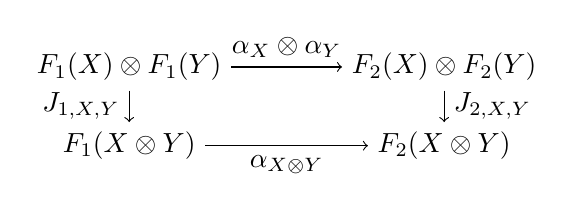
\begin{tikzpicture}
            \node (f1xf1y) at (-2,0.5) {\(F_1(X) \otimes F_1(Y)\)};
            \node (f2xf2y) at (2,0.5) {\(F_2(X) \otimes F_2(Y)\)};
            \node (f1xy) at (-2,-0.5) {\(F_1(X \otimes Y)\)};
            \node (f2xy) at (2,-0.5) {\(F_2(X \otimes Y)\)};

            \draw[->] (f1xf1y) to node[above] {\(\alpha_X \otimes \alpha_Y\)} (f2xf2y);
            \draw[->] (f1xf1y) to node[left] {\(J_{1,X,Y}\)} (f1xy);
            \draw[->] (f2xf2y) to node[right] {\(J_{2,X,Y}\)} (f2xy);
            \draw[->] (f1xy) to node[below] {\(\alpha_{X \otimes Y}\)} (f2xy);
        \end{tikzpicture}
    \end{center}
\end{definition}

\begin{corollary}
    幺半自然变换有横纵合成.

    \begin{proof}
        先验证纵合成, 以下交换图表成立:

        \begin{center}
            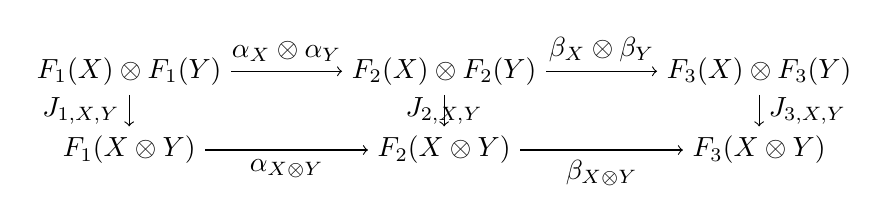
\begin{tikzpicture}
                \node (f1xf1y) at (-4,0.5) {\(F_1(X) \otimes F_1(Y)\)};
                \node (f2xf2y) at (0,0.5) {\(F_2(X) \otimes F_2(Y)\)};
                \node (f3xf3y) at (4,0.5) {\(F_3(X) \otimes F_3(Y)\)};
                \node (f1xy) at (-4,-0.5) {\(F_1(X \otimes Y)\)};
                \node (f2xy) at (0,-0.5) {\(F_2(X \otimes Y)\)};
                \node (f3xy) at (4,-0.5) {\(F_3(X \otimes Y)\)};

                \draw[->] (f1xf1y) to node[above] {\(\alpha_X \otimes \alpha_Y\)} (f2xf2y);
                \draw[->] (f2xf2y) to node[above] {\(\beta_X \otimes \beta_Y\)} (f3xf3y);
                \draw[->] (f1xf1y) to node[left] {\(J_{1,X,Y}\)} (f1xy);
                \draw[->] (f2xf2y) to node {\(J_{2,X,Y}\)} (f2xy);
                \draw[->] (f3xf3y) to node[right] {\(J_{3,X,Y}\)} (f3xy);
                \draw[->] (f1xy) to node[below] {\(\alpha_{X \otimes Y}\)} (f2xy);
                \draw[->] (f2xy) to node[below] {\(\beta_{X \otimes Y}\)} (f3xy);
            \end{tikzpicture}
        \end{center}

        再验证横合成, 验证以下交换图表成立:

        \begin{center}
            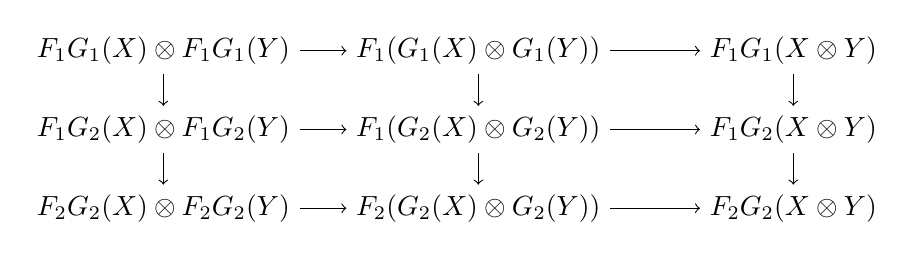
\begin{tikzpicture}
                \node (11x11y) at (-4,1) {\(F_1 G_1(X) \otimes F_1 G_1(Y)\)};
                \node (12x12y) at (-4,0) {\(F_1 G_2(X) \otimes F_1 G_2(Y)\)};
                \node (22x22y) at (-4,-1) {\(F_2 G_2(X) \otimes F_2 G_2(Y)\)};
                \node (11x1y) at (0,1) {\(F_1 (G_1(X) \otimes G_1(Y))\)};
                \node (12x2y) at (0,0) {\(F_1 (G_2(X) \otimes G_2(Y))\)};
                \node (22x2y) at (0,-1) {\(F_2 (G_2(X) \otimes G_2(Y))\)};
                \node (11xy) at (4,1) {\(F_1 G_1(X \otimes Y)\)};
                \node (12xy) at (4,0) {\(F_1 G_2(X \otimes Y)\)};
                \node (22xy) at (4,-1) {\(F_2 G_2(X \otimes Y)\)};

                \draw[->] (11x11y) to (11x1y);
                \draw[->] (12x12y) to (12x2y);
                \draw[->] (22x22y) to (22x2y);
                \draw[->] (11x11y) to (12x12y);
                \draw[->] (12x12y) to (22x22y);
                \draw[->] (11x1y) to (12x2y);
                \draw[->] (12x2y) to (22x2y);
                \draw[->] (11x1y) to (11xy);
                \draw[->] (12x2y) to (12xy);
                \draw[->] (22x2y) to (22xy);
                \draw[->] (11xy) to (12xy);
                \draw[->] (12xy) to (22xy);
            \end{tikzpicture}
        \end{center}
    \end{proof}
\end{corollary}

\begin{corollary}
    幺半自然变换的复合和自然变换享有一样的运算公式, 即横纵合成结合律与交换律.
\end{corollary}

\begin{corollary}
    幺半范畴的等价是一对幺半函子 \(F,G\) 使得其复合同构于幺半幺半范畴的恒等变换.

    \begin{proof}
        需验证其逆给出确为幺半函子, 假使有幺半函子 \(F : \mathfrak{C} \to \mathfrak{D}\), 有函子 \(G : \mathfrak{D} \to \mathfrak{C}\), 
        以及自然同构 \(\alpha : F \circ G \to \mathrm{id}_\mathfrak{D}\), \(\beta : G \circ F \to \mathrm{id}_\mathfrak{C}\),
        有 \(GX \otimes GY \xrightarrow{\beta_{X \otimes Y}^{-1}} GF (GX \otimes GY) \xrightarrow{GJ_{GX,GY}} G(FGX \otimes FGY) \xrightarrow{G(\alpha_X \otimes \alpha_Y)} GX \otimes GY\),
        可以验证上述态射使 \(G\) 成为幺半函子, 亦考察 \(\alpha,\beta\) 知复合的同构.
    \end{proof}
\end{corollary}

\subsubsection{融贯定理}

我们需说明上述 \ref{axiom:MC pentagon axiom}, \ref{axiom:MC triangle axiom}, 蕴含
所有结合与消去的交换图表都成立.

\begin{lemma}
    给出 \(n + 1\) 个有顺序的对象, 张量积时一共有 \(\frac{1}{n+1} \frac{2n!}{n!n!}\) 种打括号的方式.

    \begin{proof}
        等同于有 \(n + 1\) 个叶节点时满二叉树的数量, 记为计数函数 \(f : \mathbb{Z}_{>0} \to \mathbb{N}\),
        有 \(f(1) = 1, f(k) = \sum_{i=1}^{k-1} f(i) f(k-i)\), 递推得到 \(f(n+1) = \frac{1}{n+1} \frac{2n!}{n!n!}\).
    \end{proof}
\end{lemma}

\begin{theorem}[结合律]
    给出运算 \(R\) 满足 \(X R (Y R Z) = (X R Y) R Z\), 则括号总是可以省略.

    \begin{proof}
        我们先归纳的定义无括号时一种典范的运算顺序如下:

        \[
            X_1 R X_2 R \cdots R X_n = (X_1 R X_2) R \cdots R X_n
        \]

        归纳, 当只有三个对象时, 即为结合律本身, 假定含有 \(n\) 个对象时结合律成立, 则含有 \(n+1\) 个对象时,
        找到最外侧的 \(R\), 将该 \(R\) 右端的对象变成典范的选取, 又 \(A R (B R X_{n+1}) = (A R B) R X_{n+1}\),
        对前 \(n\) 个对象应用归纳假设, 于是得到结合律成立.
    \end{proof}
\end{theorem}

\begin{theorem}[Mac Lane 融贯定理]
    任意给出 \(n\) 个有顺序的对象与对应的张量积, 结合映射复合的结果是唯一的.

    \begin{proof}
        只需证明对于典范选取 \(X_1 \otimes X_2 \otimes \cdots \otimes X_n\) 复合到自身的结合约束是唯一的,
        对 \(n\) 进行归纳, 当 \(n = 4\) 时, 即为五边形公理, 假定 \(n = k\) 时成立, 则 \(n = k+1\) 时, 
        依赖结合律知可以典范的选取结合同态使得 \(X_{k+1}\) 在最外部.

        \[
            A \otimes B \to A \otimes (C \otimes X_{k+1}) \to (A \otimes C) \otimes X_{k+1}
        \]

        依赖于 \(B\) 包含少于 \(k + 1\) 个对象, 应用归纳假设, 上述结合约束是唯一的, 对一个最简的结合态射
        \(S \to S^\prime\), 可分类为四类情况, 第一类为 \(A \otimes B \to A^\prime \otimes B\), 第二类为
        \(A \otimes B \to A \otimes B^\prime\), 第三类为 \(A \otimes (B \otimes C) \to (A \otimes B) \otimes C\),
        第四类为 \((A \otimes B) \otimes C \to A \otimes (B \otimes C)\), 我们需证明典范的将 \(X_{k+1}\) 移动到最外部的结合态射交换.

        第一类可以展开如仪:

        \begin{center}
            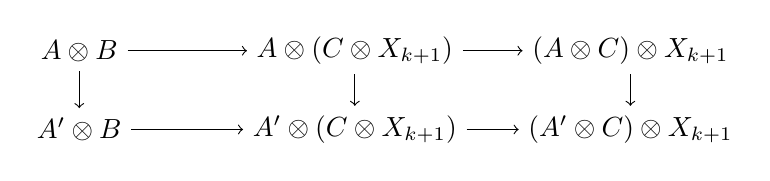
\begin{tikzpicture}
                \node (ab) at (-3.5,0.5) {\(A \otimes B\)};
                \node (acx) at (0,0.5) {\(A \otimes (C \otimes X_{k+1})\)};
                \node (apb) at (-3.5,-0.5) {\(A^\prime \otimes B\)};
                \node (apcx) at (0,-0.5) {\(A^\prime \otimes (C \otimes X_{k+1})\)};
                \node (ac) at (3.5,0.5) {\((A \otimes C) \otimes X_{k+1}\)};
                \node (apc) at (3.5,-0.5) {\((A^\prime \otimes C) \otimes X_{k+1}\)};

                \draw[->] (ab) to (acx);
                \draw[->] (ab) to (apb);
                \draw[->] (acx) to (ac);
                \draw[->] (apb) to (apcx);
                \draw[->] (acx) to (apcx);
                \draw[->] (ac) to (apc);
                \draw[->] (apcx) to (apc);
            \end{tikzpicture}
        \end{center}

        第二类无非是归纳假设, 第三类与第四类可以展开如仪, 右侧四边形即 \ref{axiom:MC pentagon axiom}.

        \begin{center}
            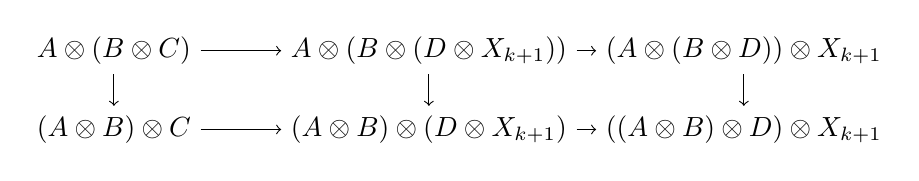
\begin{tikzpicture}
                \node (albcr) at (-4,0.5) {\(A \otimes (B \otimes C)\)};
                \node (labrc) at (-4,-0.5) {\((A \otimes B) \otimes C\)};
                \node (albdxr) at (0,0.5) {\(A \otimes (B \otimes (D \otimes X_{k+1}))\)};
                \node (labrdx) at (0,-0.5) {\((A \otimes B) \otimes (D \otimes X_{k+1})\)};
                \node (albdrx) at (4,0.5) {\((A \otimes (B \otimes D)) \otimes X_{k+1}\)};
                \node (labdrx) at (4,-0.5) {\(((A \otimes B) \otimes D) \otimes X_{k+1}\)};

                \draw[->] (albcr) to (albdxr);
                \draw[->] (albcr) to (labrc);
                \draw[->] (albdxr) to (albdrx);
                \draw[->] (labrc) to (labrdx);
                \draw[->] (albdxr) to (labrdx);
                \draw[->] (albdrx) to (labdrx);
                \draw[->] (labrdx) to (labdrx);
            \end{tikzpicture}
        \end{center}

        于是我们对任意的结合态射的复合, 都给出了以下交换图表:

        \begin{center}
            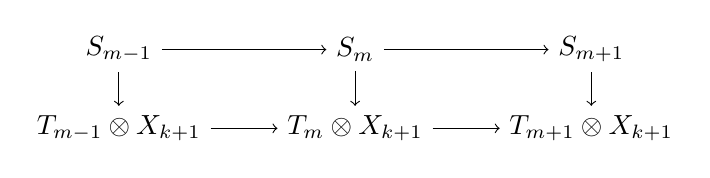
\begin{tikzpicture}
                \node (Sm) at (0,0.5) {\(S_m\)};
                \node (Sm-1) at (-3,0.5) {\(S_{m-1}\)};
                \node (Sm+1) at (3,0.5) {\(S_{m+1}\)};
                \node (Tm) at (0,-0.5) {\(T_m \otimes X_{k+1}\)};
                \node (Tm-1) at (-3,-0.5) {\(T_{m-1} \otimes X_{k+1}\)};
                \node (Tm+1) at (3,-0.5) {\(T_{m+1} \otimes X_{k+1}\)};

                \draw[->] (Sm) to (Tm);
                \draw[->] (Sm-1) to (Sm);
                \draw[->] (Sm) to (Sm+1);
                \draw[->] (Sm+1) to (Tm+1);
                \draw[->] (Tm-1) to (Tm);
                \draw[->] (Tm) to (Tm+1);
                \draw[->] (Sm-1) to (Tm-1);
            \end{tikzpicture}
        \end{center}

        依赖归纳假设, \(T_m\) 给出的结合态射是唯一的, 于是 \(S_m\) 也给出唯一的结合态射.
    \end{proof}
\end{theorem}

\begin{corollary}
    应用 \ref{axiom:MC triangle axiom}, 对 \(\mathbf{1}\) 的消去总是唯一的.
\end{corollary}

\begin{definition}[严格幺半范畴]
    一个严格幺半范畴是一个幺半范畴, 如果满足以下等式:
    \[
        \begin{aligned}
            (X \otimes Y) \otimes Z &= X \otimes (Y \otimes Z) \\
            \mathbf{1} \otimes X &= X \otimes \mathbf{1} = X
        \end{aligned}
    \]
\end{definition}

\begin{theorem}[Mac Lane 严格性定理]
    任意幺半范畴等价于一个严格幺半范畴.

    \begin{proof}
        我们构造出这样一个严格幺半范畴, 使得其在运算过程中隐含类似于上述的迁移过程.

        定义幺半范畴 \(\mathcal{V}\), 其对象为 \((F,\rho)\), 其中 \(F\) 是函子 \(\mathcal{C} \to \mathcal{C}\), 
        \(\rho\) 是自然同态 \(F(-) \otimes - \to F(- \otimes -)\), 使得以下交换图表总是成立:

        \begin{center}
            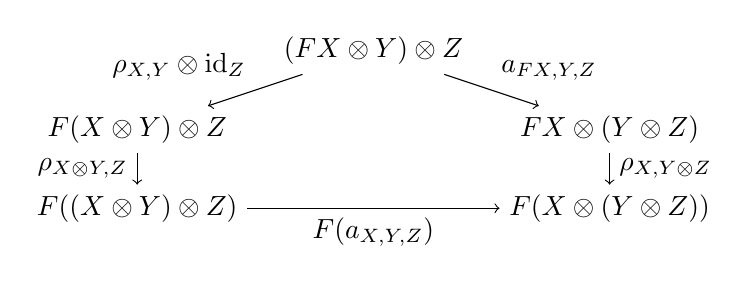
\begin{tikzpicture}
                \node (ararar) at (0,1) {\((FX \otimes Y) \otimes Z\)};
                \node (araarr) at (3,0) {\(FX \otimes (Y \otimes Z)\)};
                \node (aarrar) at (-3,0) {\(F (X \otimes Y) \otimes Z\)};
                \node (aaarrr) at (3,-1) {\(F (X \otimes (Y \otimes Z))\)};
                \node (aararr) at (-3,-1) {\(F ((X \otimes Y) \otimes Z)\)};
    
                \draw[->] (ararar) to node[above right] {\(a_{FX,Y,Z}\)} (araarr);
                \draw[->] (ararar) to node[above left] {\(\rho_{X,Y} \otimes \mathrm{id}_Z\)} (aarrar);
                \draw[->] (araarr) to node[right] {\(\rho_{X,Y \otimes Z}\)} (aaarrr);
                \draw[->] (aarrar) to node[left] {\(\rho_{X \otimes Y,Z}\)} (aararr);
                \draw[->] (aararr) to node[below] {\(F (a_{X,Y,Z})\)} (aaarrr);
            \end{tikzpicture}
        \end{center}

        其态射是与 \(\rho\) 相容的自然变换 \(\theta : F^1 \to F^2\), 使得以下交换图表成立:

        \begin{center}
            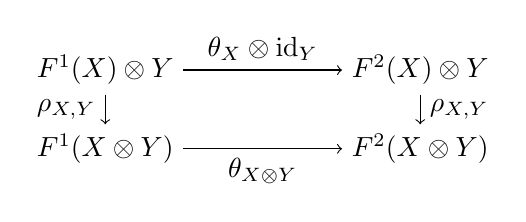
\begin{tikzpicture}
                \node (f1x) at (-2,0.5) {\(F^1(X) \otimes Y\)};
                \node (f2x) at (2,0.5) {\(F^2(X) \otimes Y\)};
                \node (f1xy) at (-2,-0.5) {\(F^1(X \otimes Y)\)};
                \node (f2xy) at (2,-0.5) {\(F^2(X \otimes Y)\)};

                \draw[->] (f1x) to node[above] {\(\theta_X \otimes \mathrm{id}_Y\)} (f2x);
                \draw[->] (f1x) to node[left] {\(\rho_{X,Y}\)} (f1xy);
                \draw[->] (f2x) to node[right] {\(\rho_{X,Y}\)} (f2xy);
                \draw[->] (f1xy) to node[below] {\(\theta_{X \otimes Y}\)} (f2xy);
            \end{tikzpicture}
        \end{center}

        给出幺元 \((\mathrm{id}_{\mathcal{C}},\mathrm{id}_{- \otimes -})\), 定义张量积为 
        \((F^1,\rho^1) \otimes (F^2,\rho^2) := (F^1 \circ F^2, (\mathrm{id}_{F^1} \ast \rho^2) \circ (\rho^1 \ast \mathrm{id}_{F^2 \times \mathrm{id}_\mathcal{C}}))\),
        显见张量积是 \(\mathcal{V} \times \mathcal{V} \to \mathcal{V}\) 的函子.

        于是有自然的嵌入 \(\psi : \mathcal{C} \to \mathcal{V}\), 使得 \(X \mapsto (X \otimes -,a_{X,-,-})\),
        态射 \(f \mapsto f \otimes \mathrm{id}_{-}\), 其与 \(\rho\) 相容源于 \(a\) 自然性.

        所定义的幺半范畴 \(\mathcal{V}\) 是严格幺半范畴, 其有唯一的三元张量积
        \((F^1,\rho^1) \otimes ((F^2,\rho^2) \otimes (F^3,\rho^3)) = (F^1 \circ F^2 \circ F^3, (\mathrm{id}_{F^1} \ast \mathrm{id}_{F^2} \ast \rho^3) \circ (\mathrm{id}_{F^1} \ast \rho^2 \ast \mathrm{id}_{F^3 \times \mathrm{id}_\mathcal{C}}) \circ (\rho^1 \ast \mathrm{id}_{(F^2 \circ F^3) \times \mathrm{id}_{\mathcal{C}}}))\)
        而对单位的消去是显见的.

        乃需验证 \(\psi\) 是幺半等价, 其函子性基于 \(a\) 自然性显然, 定义 
        \(J_{X,Y} := a_{X,Y,-} : \psi(X) \otimes \psi(Y) = (X \otimes (Y \otimes -), (\mathrm{id}_X \otimes a_{Y,-,-}) \circ a_{X,Y \otimes -,-}) \to \psi(X \otimes Y) = ((X \otimes Y) \otimes -,a_{X \otimes Y,-,-})\)
        其与 \(\rho\) 相容无非是 \ref{axiom:MC pentagon axiom}, 而 \(J\) 自然性显然. 其次, 我们考察以下图表给出的 \(F(X) \to G(X)\).

        \begin{center}
            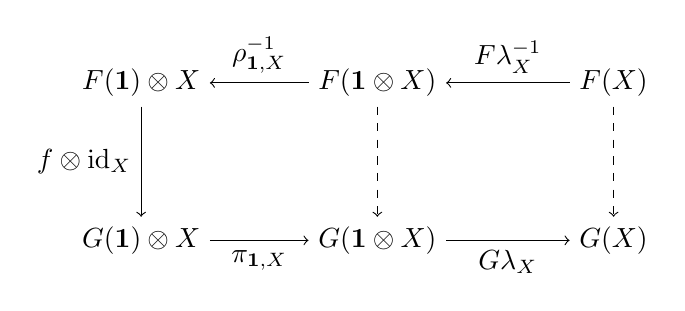
\begin{tikzpicture}
                \node (f1x) at (-3,1) {\(F(\mathbf{1}) \otimes X\)};
                \node (g1x) at (-3,-1) {\(G(\mathbf{1}) \otimes X\)};
                \node (f1xp) at (0,1) {\(F(\mathbf{1} \otimes X)\)};
                \node (g1xp) at (0,-1) {\(G(\mathbf{1} \otimes X)\)};
                \node (fx) at (3,1) {\(F(X)\)};
                \node (gx) at (3,-1) {\(G(X)\)};

                \draw[->] (fx) to node[above] {\(F \lambda_X^{-1}\)} (f1xp);
                \draw[->] (f1xp) to node[above] {\(\rho_{\mathbf{1},X}^{-1}\)} (f1x);
                \draw[->] (g1x) to node[below] {\(\pi_{\mathbf{1},X}\)} (g1xp);
                \draw[->] (g1xp) to node[below] {\(G \lambda_X\)} (gx);
                \draw[->] (f1x) to node[left] {\(f \otimes \mathrm{id}_X\)} (g1x);
                \draw[dashed,->] (f1xp) to (g1xp);
                \draw[dashed,->] (fx) to (gx);
            \end{tikzpicture}
        \end{center}

        从而 \(\mathrm{Hom}_{\mathcal{V}} ((F,\rho),(G,\pi))\) 同构于 \(\mathrm{Hom}_{\mathcal{C}} (F(\mathbf{1}),G(\mathbf{1}))\),
        该同构具自然性, 故 \(\psi\) 是等价.
    \end{proof}
\end{theorem}

上述嵌入亦称幺半米田.

\subsubsection{伴随对象}

\begin{definition}[伴随对象]
    给出幺半范畴 \(\mathcal{C}\), 某个对象 \(X\) 的左伴随是一个对象 \(X^\ast\) 若有两个态射 \(\mathrm{ev}_X : X^\ast \otimes X \to \mathbf{1}, \mathrm{coev}_X : \mathbf{1} \to X \otimes X^\ast\),
    满足等式:

    \[
        \begin{aligned}
            (\mathrm{id}_X \otimes \mathrm{ev}_X) \circ a_{X,X^\ast,X} \circ (\mathrm{coev}_X \otimes \mathrm{id}_X) &= \rho_X^{-1} \circ \lambda_X \\
            (\mathrm{ev}_X \otimes \mathrm{id}_{X^\ast}) \circ a_{X^\ast,X,X^\ast}^{-1} \circ (\mathrm{id}_{X^\ast} \otimes \mathrm{coev}_X) &= \lambda_X^{-1} \circ \rho_X 
        \end{aligned}
    \]

    右伴随是一个对象 \(^\ast X\) 若有两个态射 \(\mathrm{ev}^\prime_X : X \otimes {^\ast X} \to \mathbf{1}, \mathrm{coev}^\prime_X : \mathbf{1} \to {^\ast X} \otimes X\), 满足等式:

    \[
        \begin{aligned}
            (\mathrm{ev}^\prime_X \otimes \mathrm{id}_X) \circ a_{X,{^\ast X},X}^{-1} \circ (\mathrm{id}_X \otimes \mathrm{coev}^\prime_{X}) &= \lambda_X^{-1} \circ \rho_X \\
            (\mathrm{id}_{^\ast X} \otimes X) \circ a_{{^\ast X},X,{^\ast X}} \circ (\mathrm{coev}^\prime_X \otimes \mathrm{id}_{^\ast X}) &= \rho_X^{-1} \circ \lambda_X 
        \end{aligned}
    \]
\end{definition}

\begin{corollary}
    \({^\ast} (X^\ast) \cong X \cong {({^\ast} X)}^\ast\).
\end{corollary}

\begin{corollary}
    \(\mathbf{1}^\ast \cong {^\ast \mathbf{1}} \cong \mathbf{1}\).
\end{corollary}

\begin{corollary}
    左伴随存在则在同构意义下唯一.

    \begin{proof}
        若给出两个左伴随 \(X_1^\ast,X_2^\ast\), 略去所需的结合与消去, 有以下交换图表:

        \begin{center}
            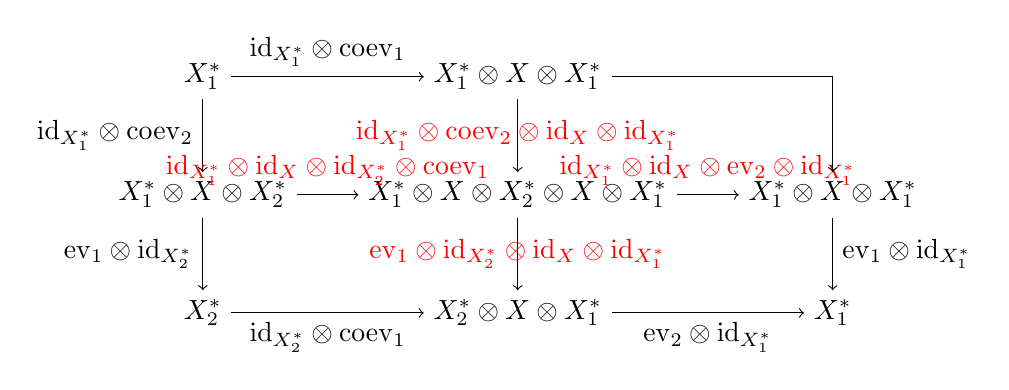
\begin{tikzpicture}
                \node (x11) at (-4,1.5) {\(X_1^\ast\)};
                \node (x2) at (-4,-1.5) {\(X_2^\ast\)};
                \node (x12) at (4,-1.5) {\(X_1^\ast\)};
                \node (x1xx2) at (-4,0) {\(X_1^\ast \otimes X \otimes X_2^\ast\)};
                \node (x1xx2xx1) at (0,0) {\(X_1^\ast \otimes X \otimes X_2^\ast \otimes X \otimes X_1^\ast\)};
                \node (x2xx1) at (0,-1.5) {\(X_2^\ast \otimes X \otimes X_1^\ast\)};
                \node (x1xx11) at (0,1.5) {\(X_1^\ast \otimes X \otimes X_1^\ast\)};
                \node (x1xx12) at (4,0) {\(X_1^\ast \otimes X \otimes X_1^\ast\)};

                \draw[->] (x11) to node[above] {\(\mathrm{id}_{X_1^\ast} \otimes \mathrm{coev}_1\)} (x1xx11);
                \draw[->] (x11) to node[left] {\(\mathrm{id}_{X_1^\ast} \otimes \mathrm{coev}_2\)} (x1xx2);
                \draw[->] (x1xx11) to node {\textcolor{red}{\(\mathrm{id}_{X_1^\ast} \otimes \mathrm{coev}_2 \otimes \mathrm{id}_X \otimes \mathrm{id}_{X_1^\ast}\)}} (x1xx2xx1);
                \draw[->] (x1xx2) to node[above] {\textcolor{red}{\(\mathrm{id}_{X_1^\ast} \otimes \mathrm{id}_X \otimes \mathrm{id}_{X_2^\ast} \otimes \mathrm{coev}_1\)}} (x1xx2xx1);
                \draw[->] (x1xx2) to node[left] {\(\mathrm{ev}_1 \otimes \mathrm{id}_{X_2^\ast}\)} (x2);
                \draw[->] (x1xx2xx1) to node[above] {\textcolor{red}{\(\mathrm{id}_{X_1^\ast} \otimes \mathrm{id}_X \otimes \mathrm{ev}_2 \otimes \mathrm{id}_{X_1^\ast}\)}} (x1xx12);
                \draw[->] (x1xx2xx1) to node {\textcolor{red}{\(\mathrm{ev}_1 \otimes \mathrm{id}_{X_2^\ast} \otimes \mathrm{id}_X \otimes \mathrm{id}_{X_1^\ast}\)}} (x2xx1);
                \draw[->] (x1xx12) to node[right] {\(\mathrm{ev}_1 \otimes \mathrm{id}_{X_1^\ast}\)} (x12);
                \draw[->] (x2) to node[below] {\(\mathrm{id}_{X_2^\ast} \otimes \mathrm{coev}_1\)} (x2xx1);
                \draw[->] (x2xx1) to node[below] {\(\mathrm{ev}_2 \otimes \mathrm{id}_{X_1^\ast}\)} (x12);
                \draw[->] (x1xx11) to (4,1.5) to (x1xx12);
            \end{tikzpicture}
        \end{center}

        同理给出对称的图表, 左上至右下合成 \(\mathrm{id}_{X_2^\ast}\), \(\mathrm{id}_{X_2^\ast}\), 于是 \((\mathrm{ev}_1 \otimes \mathrm{id}_{X_2^\ast}) \circ a_{X_1^\ast,X,X_2^\ast}^{-1} \circ (\mathrm{id}_{X_1^\ast} \otimes \mathrm{coev}_2)\) 和
        \((\mathrm{ev}_2 \otimes \mathrm{id}_{X_1^\ast}) \circ a_{X_2^\ast,X,X_1^\ast}^{-1} \circ (\mathrm{id}_{X_2^\ast} \otimes \mathrm{coev}_1)\) 给出同构.
    \end{proof}
\end{corollary}

\begin{corollary}
    右伴随存在则在同构意义下唯一.

    \begin{proof}
        证明是对称的.
    \end{proof}
\end{corollary}

\begin{definition}
    假设所论的伴随存在, 则 \(f : X \to Y\) 诱导出态射 \(f^\ast : Y^\ast \to X^\ast\) 如下:

    \begin{center}
        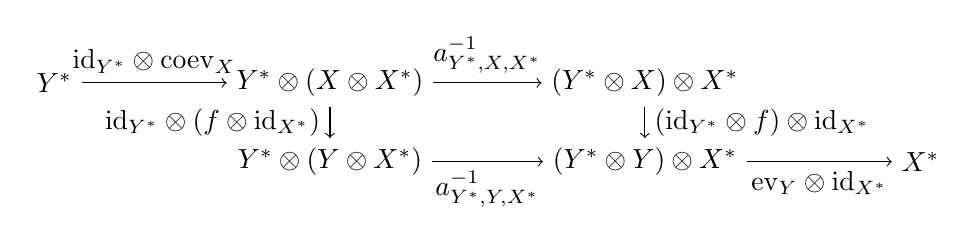
\begin{tikzpicture}
            \node (ys) at (-5.5,0.5) {\(Y^\ast\)};
            \node (ysxxs) at (-2,0.5) {\(Y^\ast \otimes (X \otimes X^\ast)\)};
            \node (ysxxsp) at (2,0.5) {\((Y^\ast \otimes X) \otimes X^\ast\)};
            \node (ysyxsp) at (-2,-0.5) {\(Y^\ast \otimes (Y \otimes X^\ast)\)};
            \node (ysyxs) at (2,-0.5) {\((Y^\ast \otimes Y) \otimes X^\ast\)};
            \node (xs) at (5.5,-0.5) {\(X^\ast\)};

            \draw[->] (ys) to node[above] {\(\mathrm{id}_{Y^\ast} \otimes \mathrm{coev}_X\)} (ysxxs);
            \draw[->] (ysxxs) to node[above] {\(a_{Y^\ast,X,X^\ast}^{-1}\)} (ysxxsp);
            \draw[->] (ysyxsp) to node[below] {\(a_{Y^\ast,Y,X^\ast}^{-1}\)} (ysyxs);
            \draw[->] (ysxxs) to node[left] {\(\mathrm{id}_{Y^\ast} \otimes (f \otimes \mathrm{id}_{X^\ast})\)} (ysyxsp);
            \draw[->] (ysxxsp) to node[right] {\((\mathrm{id}_{Y^\ast} \otimes f) \otimes \mathrm{id}_{X^\ast}\)} (ysyxs);
            \draw[->] (ysyxs) to node[below] {\(\mathrm{ev}_Y \otimes \mathrm{id}_{X^\ast}\)} (xs);
        \end{tikzpicture}
    \end{center}

    亦可定义 \(^\ast f : {^\ast Y} \to {^\ast X}\) 如下:

    \begin{center}
        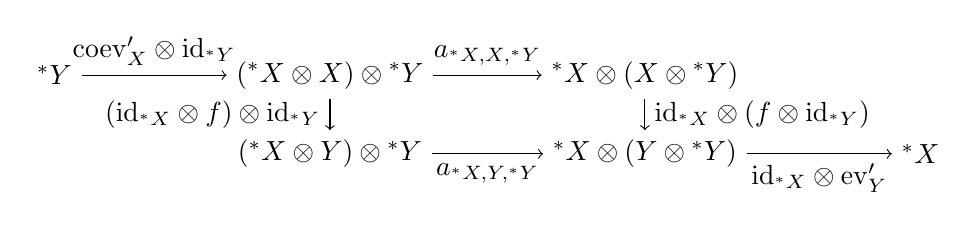
\begin{tikzpicture}
            \node (ys) at (-5.5,0.5) {\(^\ast Y\)};
            \node (xsxys) at (-2,0.5) {\(({^\ast X} \otimes X) \otimes {^\ast Y}\)};
            \node (xsxysp) at (2,0.5) {\({^\ast X} \otimes (X \otimes {^\ast Y})\)};
            \node (xsyysp) at (-2,-0.5) {\(({^\ast X} \otimes Y) \otimes {^\ast Y}\)};
            \node (xsyys) at (2,-0.5) {\({^\ast X} \otimes (Y \otimes {^\ast Y})\)};
            \node (xs) at (5.5,-0.5) {\(^\ast X\)};

            \draw[->] (ys) to node[above] {\(\mathrm{coev}^\prime_X \otimes \mathrm{id}_{^\ast Y}\)} (xsxys);
            \draw[->] (xsxys) to node[above] {\(a_{^\ast X,X,{^\ast Y}}\)} (xsxysp);
            \draw[->] (xsyysp) to node[below] {\(a_{^\ast X,Y,{^\ast Y}}\)} (xsyys);
            \draw[->] (xsxys) to node[left] {\((\mathrm{id}_{^\ast X} \otimes f) \otimes \mathrm{id}_{^\ast Y}\)} (xsyysp);
            \draw[->] (xsxysp) to node[right] {\(\mathrm{id}_{^\ast X} \otimes (f \otimes \mathrm{id}_{^\ast Y})\)} (xsyys);
            \draw[->] (xsyys) to node[below] {\(\mathrm{id}_{^\ast X} \otimes \mathrm{ev}^\prime_Y\)} (xs);
        \end{tikzpicture}
    \end{center}
\end{definition}

\begin{corollary}
    \({(f \circ g)}^\ast = g^\ast \circ f^\ast\), \(^\ast {(f \circ g)} = {^\ast g} \circ {^\ast f}\).

    \begin{proof}
        见如下给出略去结合约束的合成, 另一个方向亦然:

        \begin{center}
            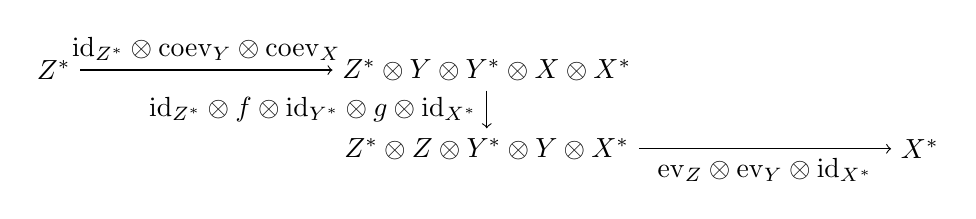
\begin{tikzpicture}
                \node (zs) at (-5.5,0.5) {\(Z^\ast\)};
                \node (xs) at (5.5,-0.5) {\(X^\ast\)};
                \node (a) at (0,0.5) {\(Z^\ast \otimes Y \otimes Y^\ast \otimes X \otimes X^\ast\)};
                \node (b) at (0,-0.5) {\(Z^\ast \otimes Z \otimes Y^\ast \otimes Y \otimes X^\ast\)};

                \draw[->] (zs) to node[above] {\(\mathrm{id}_{Z^\ast} \otimes \mathrm{coev}_Y \otimes \mathrm{coev}_X\)} (a);
                \draw[->] (a) to node[left] {\(\mathrm{id}_{Z^\ast} \otimes f \otimes \mathrm{id}_{Y^\ast} \otimes g \otimes \mathrm{id}_{X^\ast}\)} (b);
                \draw[->] (b) to node[below] {\(\mathrm{ev}_Z \otimes \mathrm{ev}_Y \otimes \mathrm{id}_{X^\ast}\)} (xs);
            \end{tikzpicture}
        \end{center}
    \end{proof}
\end{corollary}

\begin{corollary}
    给出幺半函子 \(F : \mathfrak{C} \to \mathfrak{D}\), 若 \(X\) 有左伴随 \(X^\ast\), 则 \(F(X)\) 有左伴随 \(F(X^\ast)\).

    \begin{proof}
        需给出对应的 \(\mathrm{ev},\mathrm{coev}\), 伴随性只需用 \(J,\phi\) 全部提升到 \(F\) 内部即可验证.

        \[
            \begin{aligned}
                \mathrm{ev}_{F(X)} : F(X^\ast) \otimes F(X) \xrightarrow{J_{F(X^\ast),F(X)}} F(X^\ast \otimes X) \xrightarrow{F(\mathrm{ev}_X)} F(\mathbf{1}) \xrightarrow{\phi^{-1}} \mathbf{1} \\
                \mathrm{coev}_{F(X)} : \mathbf{1} \xrightarrow{\phi} F(\mathbf{1}) \xrightarrow{F(\mathrm{coev}_X)} F(X \otimes X^\ast) \xrightarrow{J_{F(X),F(X^\ast)}^{-1}} F(X) \otimes F(X^\ast)
            \end{aligned}
        \]
    \end{proof}
\end{corollary}

\begin{corollary}
    给出幺半函子 \(F : \mathfrak{C} \to \mathfrak{D}\), 若 \(X\) 有右伴随 \(^\ast X\), 则 \(F(X)\) 有右伴随 \(^\ast F(X)\).
\end{corollary}

\begin{corollary}
    给出幺半函子 \(F : \mathfrak{C} \to \mathfrak{D}\), \(F (f)^\ast = F (f^\ast)\), \(^\ast F (f) = {^\ast F (f)}\).

    \begin{proof}
        用 \(J\) 将态射转移到 \(F\) 中.
    \end{proof}
\end{corollary}

\begin{lemma}
    若 \(X,Y\) 有左伴随 \(X^\ast,Y^\ast\), 则 \(X \otimes Y\) 有左伴随 \(Y^\ast \otimes X^\ast\).

    \begin{proof}
        给出 \(\mathrm{ev},\mathrm{coev}\) 如下:

        \[
            \begin{aligned}
                \mathrm{ev}_{X \otimes Y} : Y^\ast \otimes X^\ast \otimes X \otimes Y \xrightarrow{\mathrm{id}_{Y^\ast} \otimes \mathrm{ev}_X \otimes \mathrm{id}_Y} Y^\ast \otimes Y \xrightarrow{\mathrm{ev}_Y} \mathbf{1} \\
                \mathrm{coev}_{X \otimes Y} : \mathbf{1} \xrightarrow{\mathrm{coev}_X} X \otimes X^\ast \xrightarrow{\mathrm{id}_X \otimes \mathrm{coev}_Y \otimes \mathrm{id}_{X^\ast}} X \otimes Y \otimes Y^\ast \otimes X^\ast
            \end{aligned}
        \]

        其伴随性验证只需注意到如下略去结合约束的交换图表, 四边形交换性源于 \(\otimes\) 的函子性.

        \begin{center}
            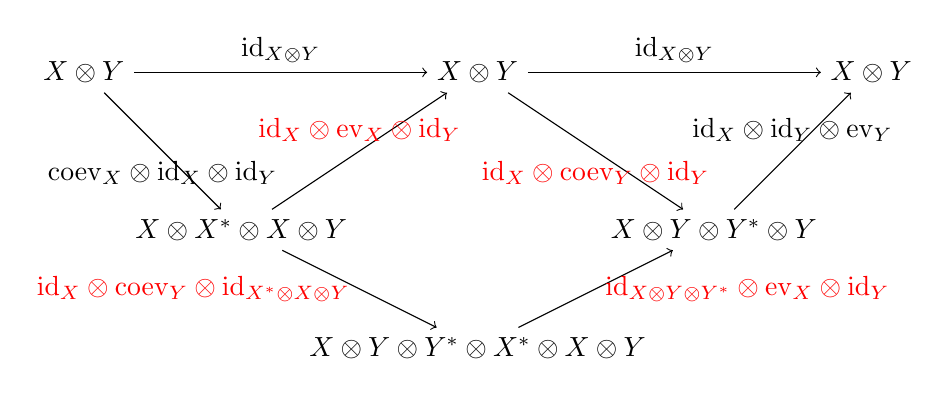
\begin{tikzpicture}
                \node (xy1) at (-5,2) {\(X \otimes Y\)};
                \node (xy2) at (0,2) {\(X \otimes Y\)};
                \node (xy3) at (5,2) {\(X \otimes Y\)};
                \node (xxxy) at (-3,0) {\(X \otimes X^\ast \otimes X \otimes Y\)};
                \node (xyyy) at (3,0) {\(X \otimes Y \otimes Y^\ast \otimes Y\)};
                \node (xyyxxy) at (0,-1.5) {\(X \otimes Y \otimes Y^\ast \otimes X^\ast \otimes X \otimes Y\)};

                \draw[->] (xy1) to node[above] {\(\mathrm{id}_{X \otimes Y}\)} (xy2);
                \draw[->] (xy2) to node[above] {\(\mathrm{id}_{X \otimes Y}\)} (xy3);
                \draw[->] (xy1) to node[below] {\(\mathrm{coev}_X \otimes \mathrm{id}_{X} \otimes \mathrm{id}_Y\)} (xxxy);
                \draw[->] (xxxy) to node[above] {\textcolor{red}{\(\mathrm{id}_X \otimes \mathrm{ev}_X \otimes \mathrm{id}_Y\)}} (xy2);
                \draw[->] (xy2) to node[below] {\textcolor{red}{\(\mathrm{id}_X \otimes \mathrm{coev}_Y \otimes \mathrm{id}_Y\)}} (xyyy);
                \draw[->] (xyyy) to node[above] {\(\mathrm{id}_X \otimes \mathrm{id}_Y \otimes \mathrm{ev}_Y\)} (xy3);
                \draw[->] (xxxy) to node[left] {\textcolor{red}{\(\mathrm{id}_X \otimes \mathrm{coev}_Y \otimes \mathrm{id}_{X^\ast \otimes X \otimes Y}\)}} (xyyxxy);
                \draw[->] (xyyxxy) to node[right] {\textcolor{red}{\(\mathrm{id}_{X \otimes Y \otimes Y^\ast} \otimes \mathrm{ev}_X \otimes \mathrm{id}_{Y}\)}} (xyyy);
            \end{tikzpicture}
        \end{center}

        \begin{center}
            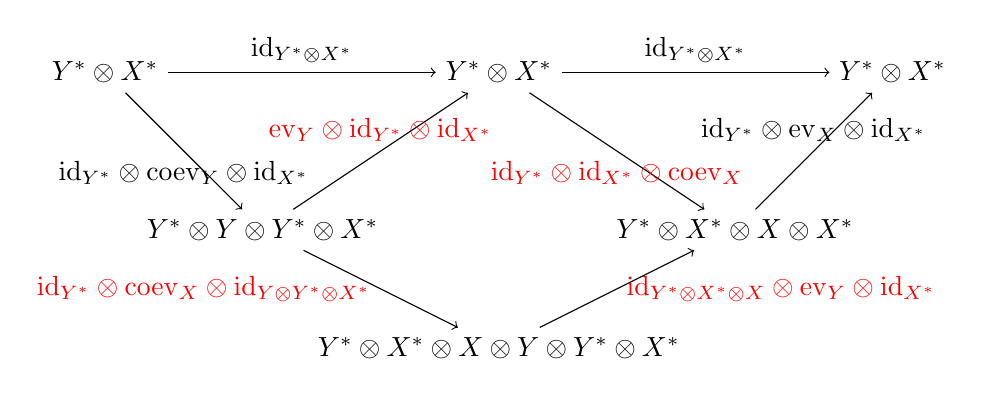
\begin{tikzpicture}
                \node (yx1) at (-5,2) {\(Y^\ast \otimes X^\ast\)};
                \node (yx2) at (0,2) {\(Y^\ast \otimes X^\ast\)};
                \node (yx3) at (5,2) {\(Y^\ast \otimes X^\ast\)};
                \node (yyyx) at (-3,0) {\(Y^\ast \otimes Y \otimes Y^\ast \otimes X^\ast\)};
                \node (yxxx) at (3,0) {\(Y^\ast \otimes X^\ast \otimes X \otimes X^\ast\)};
                \node (yxxyyx) at (0,-1.5) {\(Y^\ast \otimes X^\ast \otimes X \otimes Y \otimes Y^\ast \otimes X^\ast\)};

                \draw[->] (yx1) to node[above] {\(\mathrm{id}_{Y^\ast \otimes X^\ast}\)} (yx2);
                \draw[->] (yx2) to node[above] {\(\mathrm{id}_{Y^\ast \otimes X^\ast}\)} (yx3);
                \draw[->] (yx1) to node[below] {\(\mathrm{id}_{Y^\ast} \otimes \mathrm{coev}_Y \otimes \mathrm{id}_{X^\ast}\)} (yyyx);
                \draw[->] (yyyx) to node[above] {\textcolor{red}{\(\mathrm{ev}_Y \otimes \mathrm{id}_{Y^\ast} \otimes \mathrm{id}_{X^\ast}\)}} (yx2);
                \draw[->] (yx2) to node[below] {\textcolor{red}{\(\mathrm{id}_{Y^\ast} \otimes \mathrm{id}_{X^\ast} \otimes \mathrm{coev}_X\)}} (yxxx);
                \draw[->] (yxxx) to node[above] {\(\mathrm{id}_{Y^\ast} \otimes \mathrm{ev}_X \otimes \mathrm{id}_{X^\ast}\)} (yx3);
                \draw[->] (yyyx) to node[left] {\textcolor{red}{\(\mathrm{id}_{Y^\ast} \otimes \mathrm{coev}_X \otimes \mathrm{id}_{Y \otimes Y^\ast \otimes X^\ast}\)}} (yxxyyx);
                \draw[->] (yxxyyx) to node[right] {\textcolor{red}{\(\mathrm{id}_{Y^\ast \otimes X^\ast \otimes X} \otimes \mathrm{ev}_Y \otimes \mathrm{id}_{X^\ast}\)}} (yxxx);
            \end{tikzpicture}
        \end{center}
    \end{proof}
\end{lemma}

\begin{corollary}
    若 \(X,Y\) 有右伴随 \(^\ast X,^\ast Y\), 则 \(X \otimes Y\) 有右伴随 \(^\ast Y \otimes {^\ast X}\).
\end{corollary}

\begin{lemma}
    给出 \(V\) 的左伴随 \(V^\ast\) 就给出了伴随对 \((- \otimes V) \dashv (- \otimes V^\ast), (V^\ast \otimes -) \dashv (V \otimes -)\).

    \begin{proof}
        易于验证同构 \(\varphi : \mathrm{Hom}_{\mathcal{C}} (U \otimes V,W) \to \mathrm{Hom}_{\mathcal{C}} (U,W \otimes V^\ast)\) 如下:

        \[
            \begin{aligned}
                \varphi (f) &= (f \otimes \mathrm{id}_{V^\ast}) \circ (\mathrm{id}_U \otimes \mathrm{coev}_V) \\
                \varphi^{-1} (g) &= (\mathrm{id}_W \otimes \mathrm{ev}_V) \circ (g \otimes \mathrm{id}_V)
            \end{aligned}
        \]
    \end{proof}
\end{lemma}

\begin{corollary}
    给出 \(V\) 的右伴随 \(^\ast V\) 亦给出伴随对 \((- \otimes {^\ast V}) \dashv (- \otimes V), (V \otimes -) \dashv ({^\ast V} \otimes -)\).
\end{corollary}

\begin{corollary}
    \((-) ^{\ast \ast}, {^{\ast \ast} (-)}\) 给出幺半函子.
\end{corollary}

\begin{corollary}
    \(^\ast (f^\ast) = f\), \((^\ast f)^\ast = f\).

    \begin{proof}
        注意以下图表, 外框与右下角交换故左上角交换:

        \begin{center}
            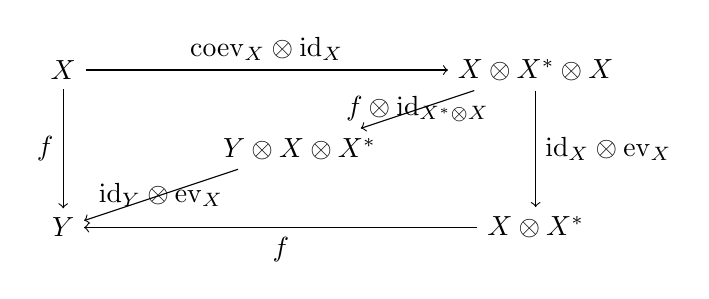
\begin{tikzpicture}
                \node (x1) at (-3,1) {\(X\)};
                \node (xxx) at (3,1) {\(X \otimes X^\ast \otimes X\)};
                \node (x2) at (3,-1) {\(X \otimes X^\ast\)};
                \node (yxx) at (0,0) {\(Y \otimes X \otimes X^\ast\)};
                \node (y) at (-3,-1) {\(Y\)};

                \draw[->] (x1) to node[above] {\(\mathrm{coev}_X \otimes \mathrm{id}_X\)} (xxx);
                \draw[->] (xxx) to node[right] {\(\mathrm{id}_X \otimes \mathrm{ev}_X\)} (x2);
                \draw[->] (x1) to node[left] {\(f\)} (y);
                \draw[->] (x2) to node[below] {\(f\)} (y);
                \draw[->] (xxx) to node {\(f \otimes \mathrm{id}_{X^\ast \otimes X}\)} (yxx);
                \draw[->] (yxx) to node {\(\mathrm{id}_Y \otimes \mathrm{ev}_X\)} (y);
            \end{tikzpicture}
        \end{center}

        于是以下图表交换:

        \begin{center}
            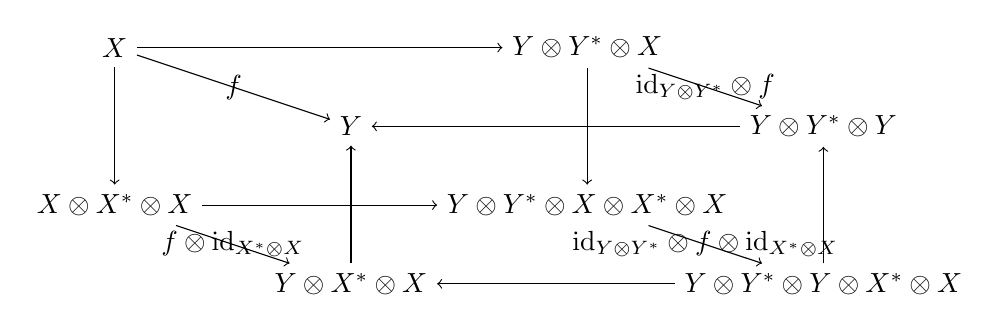
\begin{tikzpicture}
                \node (x) at (-4.5,1.5) {\(X\)};
                \node (yyx) at (1.5,1.5) {\(Y \otimes Y^\ast \otimes X\)};
                \node (xxx) at (-4.5,-0.5) {\(X \otimes X^\ast \otimes X\)};
                \node (yyxxx) at (1.5,-0.5) {\(Y \otimes Y^\ast \otimes X \otimes X^\ast \otimes X\)};
                \node (y) at (-1.5,0.5) {\(Y\)};
                \node (yyy) at (4.5,0.5) {\(Y \otimes Y^\ast \otimes Y\)};
                \node (yxx) at (-1.5,-1.5) {\(Y \otimes X^\ast \otimes X\)};
                \node (yyyxx) at (4.5,-1.5) {\(Y \otimes Y^\ast \otimes Y \otimes X^\ast \otimes X\)};

                \draw[->] (x) to (xxx);
                \draw[->] (xxx) to (yyxxx);
                \draw[->] (x) to (yyx);
                \draw[->] (yyx) to (yyxxx);
                \draw[->] (yxx) to (y);
                \draw[->] (yyyxx) to (yxx);
                \draw[->] (yyy) to (y);
                \draw[->] (yyyxx) to (yyy);
                \draw[->] (x) to node {\(f\)} (y);
                \draw[->] (yyx) to node {\(\mathrm{id}_{Y \otimes Y^\ast} \otimes f\)} (yyy);
                \draw[->] (xxx) to node {\(f \otimes \mathrm{id}_{X^\ast \otimes X}\)} (yxx);
                \draw[->] (yyxxx) to node {\(\mathrm{id}_{Y \otimes Y^\ast} \otimes f \otimes \mathrm{id}_{X^\ast \otimes X}\)} (yyyxx);
            \end{tikzpicture}
        \end{center}
    \end{proof}
\end{corollary}

\begin{definition}[刚性]
    \setlabel {刚性}
    \label {definition:rigid object in monoidal category}
    幺半范畴一个对象称为刚性的, 若其有左右伴随, 一个幺半范畴称为刚性的, 若其每个对象都是刚性的.
\end{definition}

\begin{lemma}
    给出幺半函子 \(F_1,F_2 : \mathfrak{C} \to \mathfrak{D}\) 以及幺半自然变换 \(\eta : F_1 \to F_2\), 若 \(\mathfrak{C}\)
    \ref{definition:rigid object in monoidal category}, 则 \(\eta\) 是幺半自然同构.

    \begin{proof}
        考察以下省略的交换图表, 其中三个三角形交换源自 \(\eta\) 是幺半自然变换:

        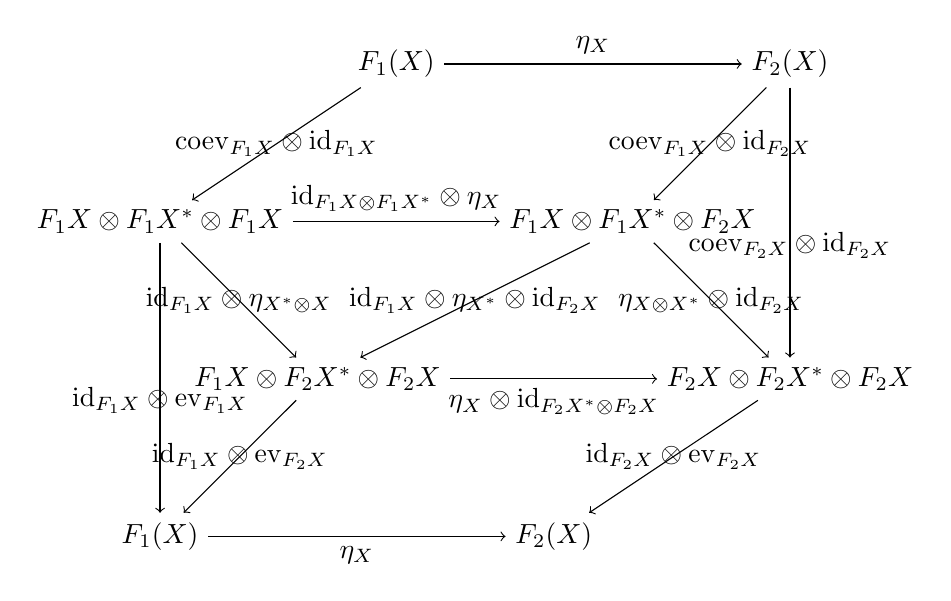
\begin{tikzpicture}
            \node (f11) at (-1,3) {\(F_1(X)\)};
            \node (f21) at (4,3) {\(F_2(X)\)};
            \node (f1f1f1) at (-4,1) {\(F_1 X \otimes F_1 X^\ast \otimes F_1 X\)};
            \node (f1f1f2) at (2,1) {\(F_1 X \otimes F_1 X^\ast \otimes F_2 X\)};
            \node (f1f2f2) at (-2,-1) {\(F_1 X \otimes F_2 X^\ast \otimes F_2 X\)};
            \node (f2f2f2) at (4,-1) {\(F_2 X \otimes F_2 X^\ast \otimes F_2 X\)};
            \node (f12) at (-4,-3) {\(F_1(X)\)};
            \node (f22) at (1,-3) {\(F_2(X)\)};

            \draw[->] (f11) to node[above] {\(\eta_X\)} (f21);
            \draw[->] (f1f1f1) to node[above] {\(\mathrm{id}_{F_1 X \otimes F_1 X^\ast} \otimes \eta_X\)} (f1f1f2);
            \draw[->] (f1f2f2) to node[below] {\(\eta_X \otimes \mathrm{id}_{F_2 X^\ast \otimes F_2 X}\)} (f2f2f2);
            \draw[->] (f12) to node[below] {\(\eta_X\)} (f22);
            \draw[->] (f11) to node {\(\mathrm{coev}_{F_1 X} \otimes \mathrm{id}_{F_1 X}\)} (f1f1f1);
            \draw[->] (f21) to node {\(\mathrm{coev}_{F_1 X} \otimes \mathrm{id}_{F_2 X}\)} (f1f1f2);
            \draw[->] (f1f1f1) to node {\(\mathrm{id}_{F_1 X} \otimes \eta_{X^\ast \otimes X}\)} (f1f2f2);
            \draw[->] (f1f1f2) to node {\(\eta_{X \otimes X^\ast} \otimes \mathrm{id}_{F_2 X}\)} (f2f2f2);
            \draw[->] (f1f2f2) to node {\(\mathrm{id}_{F_1 X} \otimes \mathrm{ev}_{F_2 X}\)} (f12);
            \draw[->] (f2f2f2) to node {\(\mathrm{id}_{F_2 X} \otimes \mathrm{ev}_{F_2 X}\)} (f22);
            \draw[->] (f1f1f1) to node[below] {\(\mathrm{id}_{F_1 X} \otimes \mathrm{ev}_{F_1 X}\)} (f12);
            \draw[->] (f21) to node[below] {\(\mathrm{coev}_{F_2 X} \otimes \mathrm{id}_{F_2 X}\)} (f2f2f2);
            \draw[->] (f1f1f2) to node {\(\mathrm{id}_{F_1 X} \otimes \eta_{X^\ast} \otimes \mathrm{id}_{F_2 X}\)} (f1f2f2);
        \end{tikzpicture}

        考察右上角 \(F_2 X\) 到左下角 \(F_1 X\) 态射, 给出了 \(\eta_X\) 的逆, 因为最左侧和最右侧合成 \(\mathrm{id}\).
    \end{proof}
\end{lemma}

\subsubsection{内 \(\mathrm{Hom}\) 对象}

\begin{definition}[内 \(\mathrm{Hom}\) 对象]
    我们称 \(\mathfrak{C}\) 有内 \(\mathrm{Hom}\) 对象, 若有函子 \(\mathrm{hom} : \mathfrak{C}^\text{op} \otimes \mathfrak{C} \to \mathfrak{C}\), 使得有自然同构:

    \[
        \mathrm{Hom}_{\mathfrak{C}} (- \otimes - , -) \to \mathrm{Hom}_{\mathfrak{C}} (-, \mathrm{hom} (-,-))
    \]
\end{definition}

\begin{definition}
    \label {definition:internal hom canonical functor}
    有如下典范的态射:

    \[
        \begin{aligned}
            \mathrm{hom} (X,Y) \otimes X &\to Y \\
            \mathrm{hom} (Y,Z) \otimes \mathrm{hom} (X,Y) &\to \mathrm{hom} (X,Z) \\
            Z \otimes \mathrm{hom} (X,Y) &\to \mathrm{hom} (X,Z \otimes Y) \\
            Y &\to \mathrm{hom} (X,Y \otimes X) \\
            \mathrm{hom} (Y,Z) \otimes X &\to \mathrm{hom} (\mathrm{hom} (X,Y),Z)
        \end{aligned}
    \]

    \begin{proof}
        我们逐个给出这些态射, 记上述自然同构为 \(\psi\).

        第一个态射为求值函数 \(\psi_{\mathrm{hom}(X,Y),X,Y}^{-1} (\mathrm{id}_{\mathrm{hom} (X,Y)})\),
        第二个态射只需注意到有两次求值 \(\mathrm{hom} (X,Y) \otimes \mathrm{hom} (Y,Z) \otimes X \to \mathrm{hom} (X,Z)\),
        第三个态射将 \(X\) 左移后仅差一求值 \(Z \otimes \mathrm{hom} (X,Y) \otimes X \to Z \otimes Y\),
        第四个态射为 \(\psi_{Y,X,X}^{-1} (\mathrm{id}_{Y \otimes X})\),
        第五个态射将 \(\mathrm{hom} (X,Y)\) 左移后为两次求值 \(\mathrm{hom} (Y,Z) \otimes \mathrm{hom} (X,Y) \otimes X \to Z\).
    \end{proof}
\end{definition}

\begin{lemma}
    每个幺半范畴 \(\mathfrak{V}\) 都可以找到一个幺半函子 \(\mathfrak{V} \to (\mathbf{Set}, \times)\),
    将对象 \(X\) 映射到 \(\mathrm{Hom}_{\mathfrak{V}} (\mathbf{1}, X)\).
\end{lemma}

\begin{lemma}
    有双射 \(\mathrm{Hom}_{\mathfrak{V}} (X,Y) \to \mathrm{Hom}_{\mathfrak{V}} (\mathbf{1}, \mathrm{hom} (X,Y))\), 此反映出了其被称为 \(\mathrm{hom}\) 的原因.
\end{lemma}

\begin{lemma}
    存在自然同构 \(i : Z \to \mathrm{hom}(\mathbf{1},Z)\).

    \begin{proof}
        令上述同构为 \(\varphi\), 考察 \(\rho_Z : Z \otimes \mathbf{1} \to Z\) 对应的态射 \(i := \varphi(\rho_Z) : Z \to \mathrm{hom} (\mathbf{1},Z)\),
        对称的考察 \(e := \varphi^{-1} (\mathrm{id}_{\mathrm{hom} (\mathbf{1},Z)}) \circ \rho_{\mathrm{hom} (\mathbf{1},Z)}^{-1} : \mathrm{hom} (\mathbf{1},Z) \to \mathrm{hom} (\mathbf{1},Z) \otimes \mathbf{1} \to Z\), 需证明其构成逆, 有:

        \[
            \begin{aligned}
                i \circ e
                &= \varphi(\rho_Z) \circ \varphi^{-1} (\mathrm{id}_{\mathrm{hom} (\mathbf{1},Z)}) \circ \rho_{\mathrm{hom} (\mathbf{1},Z)}^{-1} \\
                &= \varphi (\rho_Z \circ (\varphi^{-1} (\mathrm{id}_{\mathrm{hom} (\mathbf{1},Z)} \otimes \mathrm{id}_{\mathbf{1}}) \circ (\rho_{\mathrm{hom} (\mathbf{1},Z)}^{-1})) \otimes \mathrm{id}_{\mathbf{1}}) \\
                &= \varphi (\varphi^{-1} (\mathrm{id}_{\mathrm{hom} (\mathbf{1},Z)})) = \mathrm{id}_{\mathrm{hom} (\mathbf{1},Z)} \\
                (e \circ i) \otimes \mathrm{id}_{\mathbf{1}} \otimes \mathrm{id}_{\mathbf{1}}
                &= (\varphi^{-1} (\mathrm{id}_{\mathrm{hom} (\mathbf{1},Z)}) \circ \rho_{\mathrm{hom} (\mathbf{1},Z)}^{-1} \circ \varphi(\rho_Z)) \otimes \mathrm{id}_{\mathbf{1}} \otimes \mathrm{id}_{\mathbf{1}} \\
                &= (\varphi^{-1} (\mathrm{id}_{\mathrm{hom} (\mathbf{1},Z)}) \circ (\mathrm{id}_{\mathrm{hom} (\mathbf{1},Z)} \otimes \mathrm{id}_{\mathbf{1}}) \circ (\varphi(\rho_Z) \otimes \mathrm{id}_{\mathbf{1}})) \otimes \iota^{-1} \\
                &= (\varphi^{-1} (\varphi (\rho_Z))) \otimes \iota^{-1} = \mathrm{id}_Z \otimes \mathrm{id}_{\mathbf{1}} \otimes \mathrm{id}_{\mathbf{1}} \\
            \end{aligned}
        \]
    \end{proof}
\end{lemma}

\begin{lemma}
    有同构 \(\mathrm{hom} (X \otimes Y,Z) \to \mathrm{hom} (X,\mathrm{hom} (Y,Z))\).

    \begin{proof}
        \ref{lemma:Yoneda lemma}.
    \end{proof}
\end{lemma}

\begin{definition}
    \setlabel {双边闭}
    \label {definition:biclosed monoidal category}
    假使 \(\mathfrak{C}\) 有内 \(\mathrm{Hom}\) 对象, 对称对每个 \(X\) 亦给出 \(X \otimes -\) 的右伴随,
    且对 \(X\) 有函子性, 则称 \(\mathfrak{C}\) 为双边闭的.
\end{definition}

\subsubsection{可逆元}

\begin{definition}[可逆元]
    \setlabel {可逆}
    \label {definition:invertible element in monoidal category}
    \ref{definition:rigid object in monoidal category} 幺半范畴中一个对象 \(X\) 称为可逆的, 若 \(\mathrm{ev}_X, \mathrm{coev}_X\) 是同构.
\end{definition}

\begin{lemma}
    可逆元的左伴随同构于右伴随.

    \begin{proof}
        \(^\ast X \cong {^\ast X} \otimes X \otimes X^\ast \cong X^\ast\).
    \end{proof}
\end{lemma}

\begin{lemma}
    可逆元 \(X,Y\) 的积 \(X \otimes Y\) 亦可逆.

    \begin{proof}
        \(X \otimes Y \otimes Y^\ast \otimes X^\ast \cong X \otimes X^\ast \cong \mathbf{1}\),
        \(Y^\ast \otimes X^\ast \otimes X \otimes Y \cong Y^\ast \otimes Y \cong \mathbf{1}\).
    \end{proof}
\end{lemma}

\begin{definition}
    全体可逆元构成子幺半范畴 \(\mathrm{inv} (\mathfrak{C})\).
\end{definition}

\begin{definition}
    \(\mathrm{Gr}\) 范畴是 \ref{definition:rigid object in monoidal category} 所有元素可逆且所有态射可逆的幺半范畴.
\end{definition}

\subsection{充实范畴 (Unfinished)}

\subsubsection{基本定义}

\begin{definition}[充实范畴]
    \label {definition:enriched category}
    给定一个幺半范畴 \(\mathfrak{V}\), 一个 \(\mathfrak{V}\) - 充实范畴是一个范畴 \(\mathcal{C}\), 
    使得每个 \(\mathrm{Hom}_{\mathcal{C}} (X,Y)\) 是一个 \(\mathfrak{V}\) 的对象 \(\mathrm{hom} (X,Y)\),
    并且给出复合规则 \(M_{X,Y,Z} : \mathrm{hom}_{\mathcal{C}} (Y,Z) \otimes \mathrm{hom}_{\mathcal{C}} (X,Y) \to \mathrm{hom}_{\mathcal{C}} (X,Z)\),
    与单位规则 \(j_X : \mathbf{1} \to \mathrm{hom}_{\mathcal{C}} (X,X)\),
    满足五边形公理和三角形公理.
    \setlabel {五边形公理}
    \label {axiom:pentagon axiom in enriched category}

    \begin{center}
        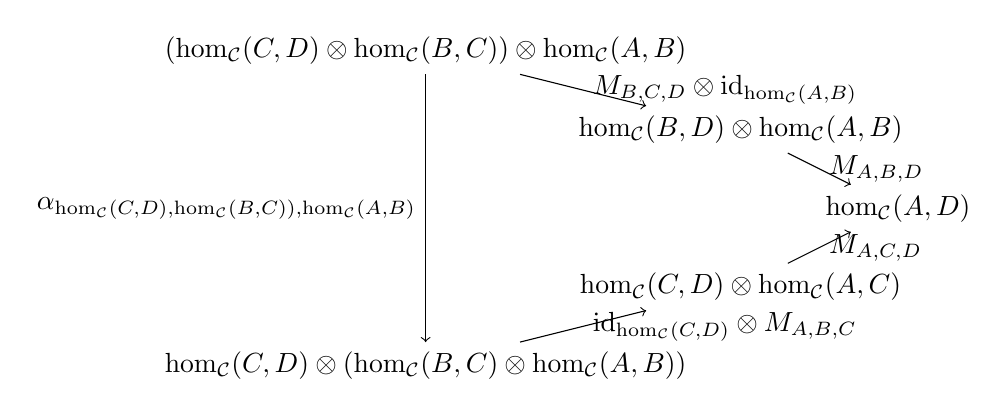
\begin{tikzpicture}
            \node (lxoyroz) at (-3,2) {\((\mathrm{hom}_{\mathcal{C}} (C,D) \otimes \mathrm{hom}_{\mathcal{C}} (B,C)) \otimes \mathrm{hom}_{\mathcal{C}} (A,B)\)};
            \node (xolyozr) at (-3,-2) {\(\mathrm{hom}_{\mathcal{C}} (C,D) \otimes (\mathrm{hom}_{\mathcal{C}} (B,C) \otimes \mathrm{hom}_{\mathcal{C}} (A,B))\)};
            \node (xyoz) at (1,1) {\(\mathrm{hom}_{\mathcal{C}} (B,D) \otimes \mathrm{hom}_{\mathcal{C}} (A,B)\)};
            \node (xoyz) at (1,-1) {\(\mathrm{hom}_{\mathcal{C}} (C,D) \otimes \mathrm{hom}_{\mathcal{C}} (A,C)\)};
            \node (xyz) at (3,0) {\(\mathrm{hom}_{\mathcal{C}} (A,D)\)};

            \draw[->] (lxoyroz) to node[left] {\(\alpha_{\mathrm{hom}_{\mathcal{C}} (C,D),\mathrm{hom}_{\mathcal{C}} (B,C)),\mathrm{hom}_{\mathcal{C}} (A,B)}\)} (xolyozr);
            \draw[->] (lxoyroz) to node[right] {\(M_{B,C,D} \otimes \mathrm{id}_{\mathrm{hom}_{\mathcal{C}} (A,B)}\)} (xyoz);
            \draw[->] (xolyozr) to node[right] {\(\mathrm{id}_{\mathrm{hom}_{\mathcal{C}} (C,D)} \otimes M_{A,B,C}\)} (xoyz);
            \draw[->] (xyoz) to node[right] {\(M_{A,B,D}\)} (xyz);
            \draw[->] (xoyz) to node[right] {\(M_{A,C,D}\)} (xyz);
        \end{tikzpicture}
    \end{center}

    \setlabel {三角形公理}
    \label {axiom:triangle axiom in enriched category}

    \begin{center}
        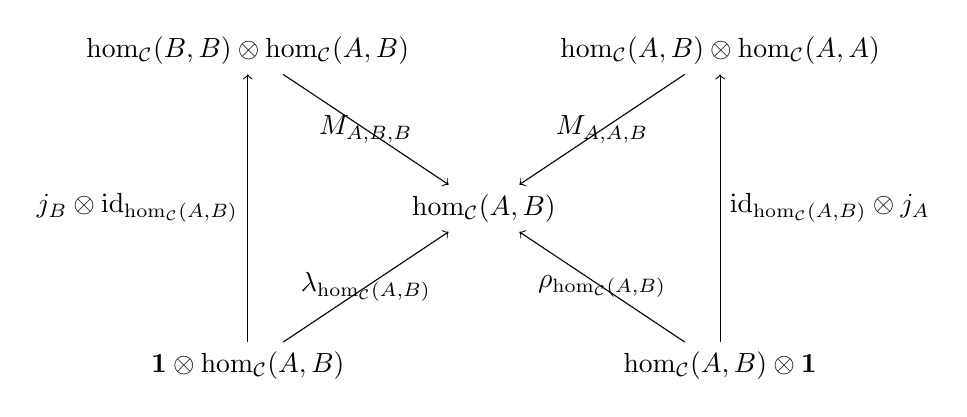
\begin{tikzpicture}
            \node (ab) at (0,0) {\(\mathrm{hom}_{\mathcal{C}} (A,B)\)};
            \node (bbab) at (-3,2) {\(\mathrm{hom}_{\mathcal{C}} (B,B) \otimes \mathrm{hom}_{\mathcal{C}} (A,B)\)};
            \node (abaa) at (3,2) {\(\mathrm{hom}_{\mathcal{C}} (A,B) \otimes \mathrm{hom}_{\mathcal{C}} (A,A)\)};
            \node (iab) at (-3,-2) {\(\mathbf{1} \otimes \mathrm{hom}_{\mathcal{C}} (A,B)\)};
            \node (abi) at (3,-2) {\(\mathrm{hom}_{\mathcal{C}} (A,B) \otimes \mathbf{1}\)};

            \draw[->] (bbab) to node {\(M_{A,B,B}\)} (ab);
            \draw[->] (abaa) to node {\(M_{A,A,B}\)} (ab);
            \draw[->] (iab) to node[left] {\(j_B \otimes \mathrm{id}_{\mathrm{hom}_{\mathcal{C}} (A,B)}\)} (bbab);
            \draw[->] (abi) to node[right] {\(\mathrm{id}_{\mathrm{hom}_{\mathcal{C}} (A,B)} \otimes j_A\)} (abaa);
            \draw[->] (iab) to node {\(\lambda_{\mathrm{hom}_{\mathcal{C}} (A,B)}\)} (ab);
            \draw[->] (abi) to node {\(\rho_{\mathrm{hom}_{\mathcal{C}} (A,B)}\)} (ab);
        \end{tikzpicture}
    \end{center}
\end{definition}

\begin{definition}
    一个 \(2\) - 范畴定义上与严格 \(2\) - 范畴相差无几, 但 \(1\) - 态射的复合不再是结合的, 而给出自然的 \(2\) - 态射:

    \[
        \alpha_{f,g,h} : (h \circ g) \circ f \to h \circ (g \circ f), \lambda_f : f \circ \mathrm{id} \to f, \rho_f : \mathrm{id} \circ f \to f
    \]

    满足五边形公理和三角形公理.

    \[
        \alpha_{f,g,i \circ h} \circ (\alpha_{f \circ g,h,i}) = (\mathrm{id}_i \ast \alpha_{h,g,f}) \circ \alpha_{f,h \circ g,i} \circ (\alpha_{g,h,i} \ast \mathrm{id}_f)
    \]

    \[
        (\mathrm{id}_{\mathrm{id}} \ast \lambda_f) \circ \alpha_{f,\mathrm{id},g} = (\rho_{g} \ast \mathrm{id}_f)
    \]
\end{definition}

\begin{remark}
    \(2\) - 范畴即 \((\mathbf{Cat}, \otimes := \times)\) - 充实范畴.
\end{remark}

\begin{corollary}
    \((\mathbf{Set}, \otimes := \times)\) - 充实范畴就是普通的范畴.
\end{corollary}

\begin{remark}
    上述 \ref{axiom:pentagon axiom in enriched category} 与 \ref{axiom:triangle axiom in enriched category} 使得 \(M\) 总是与结合和消去交换,
    故以下叙述中常略去二者.

    \begin{proof}
        任意打括号有唯一的 \(M : \mathrm{hom}_\mathcal{C} (A_{n-1},A_n) \otimes \cdots \otimes \mathrm{hom}_\mathcal{C} (A_0,A_1) \to \mathrm{hom}_{\mathcal{C}} (A_0,A_n)\),
        使得 \(M\) 的合成不包含结合同构, 也即对于满二叉树每次将 \({{\bullet},{\bullet}}\) 替换为 \({\bullet}\),
        依赖 \(\otimes\) 函子性, 可以替换顺序的操作总是交换的.

        只需验证 \(a\) 与 \(M\) 的交换, 而这就是 \ref{axiom:pentagon axiom in enriched category}.
    \end{proof}
\end{remark}

\begin{definition}
    一个 \(\mathfrak{V}\) - 函子 \(T\) 是一个 \(\mathfrak{V}\) - 充实范畴 \(\mathcal{C}\) 到另一个 \(\mathfrak{V}\) - 充实范畴 \(\mathcal{D}\) 的对象集上的映射 \(T : \mathrm{Ob} (\mathcal{C}) \to \mathrm{Ob} (\mathcal{D})\) 与
    一族态射 \(T_{A,B} : \mathrm{hom}_{\mathcal{C}} (A,B) \to \mathrm{hom}_{\mathcal{D}} (TA,TB)\), 使得以下图表交换:

    \begin{center}
        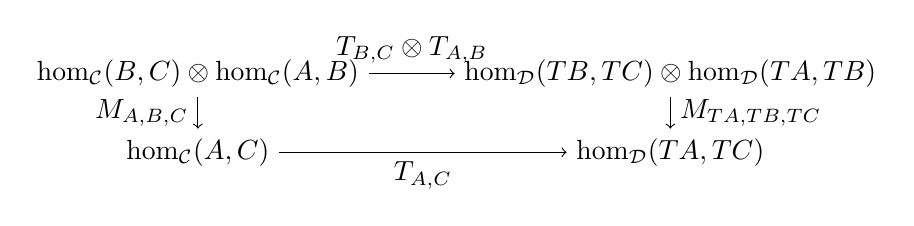
\begin{tikzpicture}
            \node (c2) at (-3,0.5) {\(\mathrm{hom}_{\mathcal{C}} (B,C) \otimes \mathrm{hom}_{\mathcal{C}} (A,B)\)};
            \node (c1) at (-3,-0.5) {\(\mathrm{hom}_{\mathcal{C}} (A,C)\)};
            \node (d2) at (3,0.5) {\(\mathrm{hom}_{\mathcal{D}} (TB,TC) \otimes \mathrm{hom}_{\mathcal{D}} (TA,TB)\)};
            \node (d1) at (3,-0.5) {\(\mathrm{hom}_{\mathcal{D}} (TA,TC)\)};

            \draw[->] (c2) to node[left] {\(M_{A,B,C}\)} (c1);
            \draw[->] (d2) to node[right] {\(M_{TA,TB,TC}\)} (d1);
            \draw[->] (c2) to node[above] {\(T_{B,C} \otimes T_{A,B}\)} (d2);
            \draw[->] (c1) to node[below] {\(T_{A,C}\)} (d1);
        \end{tikzpicture}
    \end{center}

    \begin{center}
        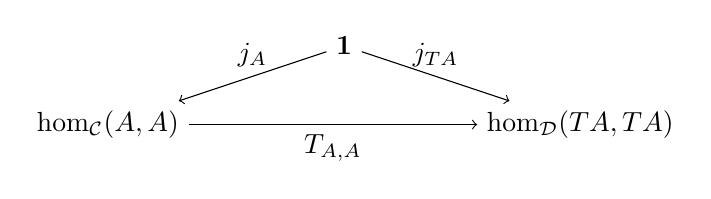
\begin{tikzpicture}
            \node (1) at (0,0.5) {\(\mathbf{1}\)};
            \node (c) at (-3,-0.5) {\(\mathrm{hom}_{\mathcal{C}} (A,A)\)};
            \node (d) at (3,-0.5) {\(\mathrm{hom}_{\mathcal{D}} (TA,TA)\)};

            \draw[->] (1) to node[above] {\(j_A\)} (c);
            \draw[->] (1) to node[above] {\(j_{TA}\)} (d);
            \draw[->] (c) to node[below] {\(T_{A,A}\)} (d);
        \end{tikzpicture}
    \end{center}
\end{definition}

\begin{definition}
    一个 \(\mathfrak{V}\) - 自然变换定义于两个 \(\mathfrak{V}\) - 函子 \(T,S : \mathcal{C} \to \mathcal{D}\) 之间,
    是一个族 \(\eta_A : \mathbf{1} \to \mathrm{hom}_{\mathcal{D}} (TA,SA)\), 使得以下图表交换:

    \begin{center}
        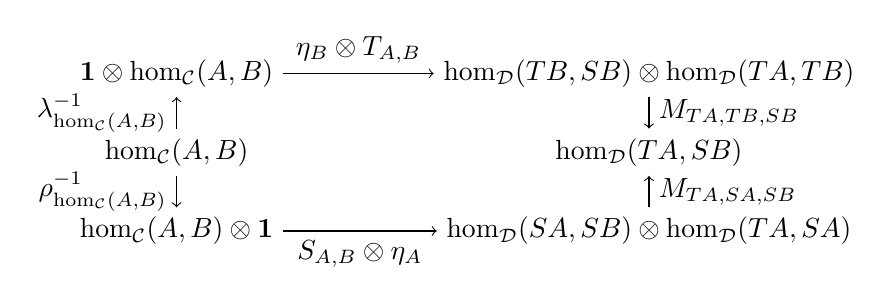
\begin{tikzpicture}
            \node (ab) at (-3,0) {\(\mathrm{hom}_{\mathcal{C}} (A,B)\)};
            \node (iab) at (-3,1) {\(\mathbf{1} \otimes \mathrm{hom}_{\mathcal{C}} (A,B)\)};
            \node (abi) at (-3,-1) {\(\mathrm{hom}_{\mathcal{C}} (A,B) \otimes \mathbf{1}\)};
            \node (diab) at (3,1) {\(\mathrm{hom}_{\mathcal{D}} (TB,SB) \otimes \mathrm{hom}_{\mathcal{D}} (TA,TB)\)};
            \node (dabi) at (3,-1) {\(\mathrm{hom}_{\mathcal{D}} (SA,SB) \otimes \mathrm{hom}_{\mathcal{D}} (TA,SA)\)};
            \node (dab) at (3,0) {\(\mathrm{hom}_{\mathcal{D}} (TA,SB)\)};

            \draw[->] (ab) to node[left] {\(\lambda_{\mathrm{hom}_{\mathcal{C}} (A,B)}^{-1}\)} (iab);
            \draw[->] (ab) to node[left] {\(\rho_{\mathrm{hom}_{\mathcal{C}} (A,B)}^{-1}\)} (abi);
            \draw[->] (iab) to node[above] {\(\eta_B \otimes T_{A,B}\)} (diab);
            \draw[->] (abi) to node[below] {\(S_{A,B} \otimes \eta_A\)} (dabi);
            \draw[->] (diab) to node[right] {\(M_{TA,TB,SB}\)} (dab);
            \draw[->] (dabi) to node[right] {\(M_{TA,SA,SB}\)} (dab);
        \end{tikzpicture}
    \end{center}
\end{definition}

\begin{definition}
    寻此思路可以归纳定义 \(n - \mathbf{Cat}_{Strict}\) 为全体严格 \(n\) - 范畴, 
    只需取 \(0 - \mathbf{Cat}_{Strict} := \mathbf{Set}\), \((n+1) - \mathbf{Cat}_{Strict} := (n - \mathbf{Cat}_{Strict})\) - 充实范畴.
\end{definition}

\begin{definition}[纵合成]
    给出两个 \(\mathfrak{V}\) - 自然变换 \(\eta : T \to S, \theta : S \to R\), 我们定义纵合成 \(\theta \circ \eta : T \to R\) 为:
    \({(\theta \circ \eta)}_A := M_{TA,SA,RA} \circ (\theta_A \otimes \eta_A) \circ \iota^{-1}\).

    \begin{proof}
        略去结合和单位的检验, 有以下交换图表:

        \begin{center}
            \begin{tikzpicture}[font = \tiny]
                \node (cab) at (-5,0) {\(\mathrm{hom}_{\mathcal{C}} (A,B)\)};
                \node (dab) at (4.5,0) {\(\mathrm{hom}_{\mathcal{D}} (TA,RB)\)};
                \node (bb) at (-2.5,2) {\(\mathrm{hom}_{\mathcal{D}} (SB,RB) \otimes \mathrm{hom}_{\mathcal{D}} (TB,SB) \otimes \mathrm{hom}_{\mathcal{D}} (TA,TB)\)};
                \node (ba) at (-0.5,0) {\(\mathrm{hom}_{\mathcal{D}} (SB,RB) \otimes \mathrm{hom}_{\mathcal{D}} (SA,SB) \otimes \mathrm{hom}_{\mathcal{D}} (TA,SA)\)};
                \node (aa) at (-2.5,-2) {\(\mathrm{hom}_{\mathcal{D}} (RA,RB) \otimes \mathrm{hom}_{\mathcal{D}} (SA,RA) \otimes \mathrm{hom}_{\mathcal{D}} (TA,SA)\)};
                \node (sbrb) at (-0.5,1) {\(\mathrm{hom}_{\mathcal{D}} (SB,RB) \otimes \mathrm{hom}_{\mathcal{D}} (TA,SB)\)};
                \node (tasa) at (-0.5,-1) {\(\mathrm{hom}_{\mathcal{D}} (SA,RB) \otimes \mathrm{hom}_{\mathcal{D}} (TA,SA)\)};
                \node (tatb) at (3,1.5) {\(\mathrm{hom}_{\mathcal{D}} (TB,RB) \otimes \mathrm{hom}_{\mathcal{D}} (TA,TB)\)};
                \node (rarb) at (3,-1.5) {\(\mathrm{hom}_{\mathcal{D}} (RA,RB) \otimes \mathrm{hom}_{\mathcal{D}} (TA,RA)\)};

                \draw[->] (cab) to node[left] {\(\theta_B \otimes \eta_B \otimes T_{A,B}\)} (bb);
                \draw[->] (cab) to node[left] {\(R_{A,B} \otimes \theta_A \otimes \eta_A\)} (aa);
                \draw[->] (cab) to node[below] {\(\theta_B \otimes \eta_A\)} (ba);
                \draw[->] (bb) to node {\(\mathrm{id}_{\mathrm{hom}_{\mathcal{D}} (SB,RB)} \otimes M_{TA,TB,SB}\)} (sbrb);
                \draw[->] (aa) to node {\(M_{SA,RA,RB} \otimes \mathrm{id}_{\mathrm{hom}_{\mathcal{D}} (TA,SA)}\)} (tasa);
                \draw[->] (ab) to node {\(\mathrm{id}_{\mathrm{hom}_{\mathcal{D}} (SB,RB)} \otimes M_{TA,SA,SB}\)} (sbrb);
                \draw[->] (ab) to node {\(M_{SA,SB,RB} \otimes \mathrm{id}_{\mathrm{hom}_{\mathcal{D}} (TA,SA)}\)} (tasa);
                \draw[->] (bb) to node[above right] {\(M_{TB,SB,RB} \otimes \mathrm{id}_{\mathrm{hom}_{\mathcal{D}} (TA,TB)}\)} (tatb);
                \draw[->] (aa) to node[below right] {\(\mathrm{id}_{\mathrm{hom}_{\mathcal{D}} (RA,RB)} \otimes M_{TA,SA,RA}\)} (rarb);
                \draw[->] (sbrb) to node {\(M_{TA,SB,RB}\)} (dab);
                \draw[->] (tasa) to node {\(M_{TA,SA,RB}\)} (dab);
                \draw[->] (tatb) to node {\(M_{TA,TB,RB}\)} (dab);
                \draw[->] (rarb) to node {\(M_{TA,RA,RB}\)} (dab);
            \end{tikzpicture}
        \end{center}

        其中右侧四个四边形交换源自于 \ref{axiom:pentagon axiom in enriched category}.
    \end{proof}
\end{definition}

\begin{definition}[函子合成]
    给出两个 \(\mathfrak{V}\) - 函子 \(T : \mathcal{C} \to \mathcal{D}, S : \mathcal{D} \to \mathcal{E}\), 我们定义函子合成 \(S \circ T : \mathcal{C} \to \mathcal{E}\),
    其在对象集上的作用为 \(S \circ T (X) := S(T(X))\), 而给出 \({(S \circ T)}_{A,B} : S_{TA,TB} \circ T_{A,B}\).

    \begin{proof}
        注意到 \(\otimes\) 函子性下图左边一列给出 \({(S \circ T)}_{B,C} \otimes {(S \circ T)}_{A,B}\).

        \begin{center}
            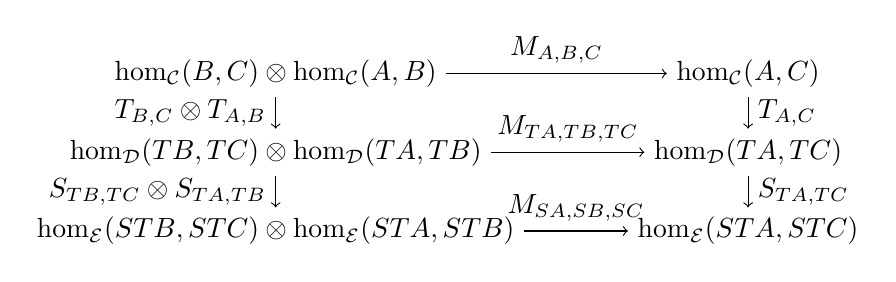
\begin{tikzpicture}
                \node (abc) at (-3,1) {\(\mathrm{hom}_{\mathcal{C}} (B,C) \otimes \mathrm{hom}_{\mathcal{C}} (A,B)\)};
                \node (ac) at (3,1) {\(\mathrm{hom}_{\mathcal{C}} (A,C)\)};
                \node (tabc) at (-3,0) {\(\mathrm{hom}_{\mathcal{D}} (TB,TC) \otimes \mathrm{hom}_{\mathcal{D}} (TA,TB)\)};
                \node (tac) at (3,0) {\(\mathrm{hom}_{\mathcal{D}} (TA,TC)\)};
                \node (stabc) at (-3,-1) {\(\mathrm{hom}_{\mathcal{E}} (STB,STC) \otimes \mathrm{hom}_{\mathcal{E}} (STA,STB)\)};
                \node (stac) at (3,-1) {\(\mathrm{hom}_{\mathcal{E}} (STA,STC)\)};

                \draw[->] (abc) to node[left] {\(T_{B,C} \otimes T_{A,B}\)} (tabc);
                \draw[->] (ac) to node[right] {\(T_{A,C}\)} (tac);
                \draw[->] (tabc) to node[left] {\(S_{TB,TC} \otimes S_{TA,TB}\)} (stabc);
                \draw[->] (tac) to node[right] {\(S_{TA,TC}\)} (stac);
                \draw[->] (abc) to node[above] {\(M_{A,B,C}\)} (ac);
                \draw[->] (tabc) to node[above] {\(M_{TA,TB,TC}\)} (tac);
                \draw[->] (stabc) to node[above] {\(M_{SA,SB,SC}\)} (stac);
            \end{tikzpicture}
        \end{center}

        \begin{center}
            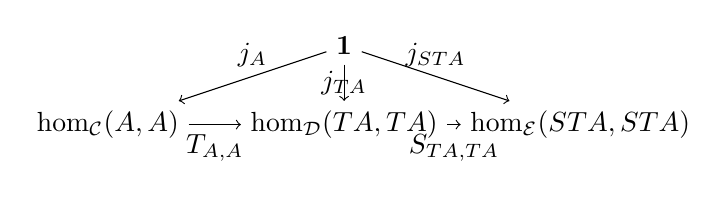
\begin{tikzpicture}
                \node (1) at (0,0.5) {\(\mathbf{1}\)};
                \node (c) at (-3,-0.5) {\(\mathrm{hom}_{\mathcal{C}} (A,A)\)};
                \node (d) at (0,-0.5) {\(\mathrm{hom}_{\mathcal{D}} (TA,TA)\)};
                \node (e) at (3,-0.5) {\(\mathrm{hom}_{\mathcal{E}} (STA,STA)\)};

                \draw[->] (1) to node[above] {\(j_A\)} (c);
                \draw[->] (1) to node {\(j_{TA}\)} (d);
                \draw[->] (1) to node[above] {\(j_{STA}\)} (e);
                \draw[->] (c) to node[below] {\(T_{A,A}\)} (d);
                \draw[->] (d) to node[below] {\(S_{TA,TA}\)} (e);
            \end{tikzpicture}
        \end{center}
    \end{proof}
\end{definition}

\begin{corollary}
    显见函子合成满足结合律.
\end{corollary}

\begin{definition}[横合成]
    给出两个 \(\mathfrak{V}\) - 自然变换 \(\eta : T \to S, \theta : U \to V\), 我们定义横合成 \(\theta \ast \eta : U \circ T \to V \circ S\) 为:
    \(M_{UTA,USA,VSA} \circ (\theta_{SA} \otimes (U_{TA,SA} \circ \eta_A)) \circ \iota^{-1} = M_{UTA,VTA,VSA} \circ ((V_{TA,SA} \circ \eta_A) \otimes \theta_{TA}) \circ \iota^{-1}\).

    \begin{proof}
        先验证定义中提到的等式 \(M_{UTA,USA,VSA} \circ (\theta_{SA} \otimes (U_{TA,SA} \circ \eta_A)) = M_{UTA,VTA,VSA} \circ ((V_{TA,SA} \circ \eta_A) \otimes \theta_{TA})\),
        施 \(\theta\) 自然性于 \(\eta_A\) 可得以下图表:

        \begin{center}
            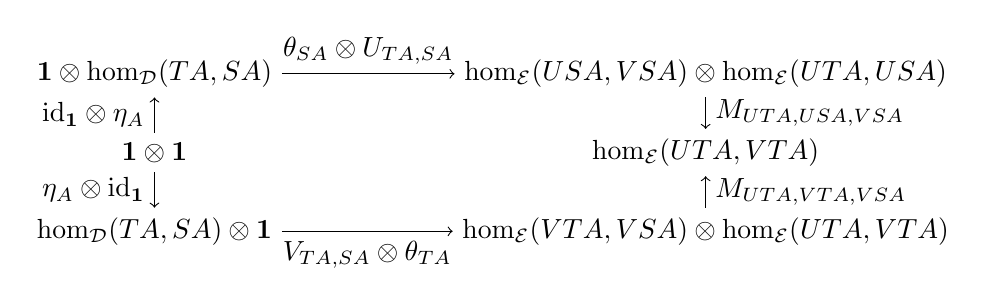
\begin{tikzpicture}
                \node (1) at (-3.5,0) {\(\mathbf{1} \otimes \mathbf{1}\)};
                \node (1ts) at (-3.5,1) {\(\mathbf{1} \otimes \mathrm{hom}_{\mathcal{D}} (TA,SA)\)};
                \node (ts1) at (-3.5,-1) {\(\mathrm{hom}_{\mathcal{D}} (TA,SA) \otimes \mathbf{1}\)};
                \node (uu) at (3.5,1) {\(\mathrm{hom}_{\mathcal{E}} (USA,VSA) \otimes \mathrm{hom}_{\mathcal{E}} (UTA,USA)\)};
                \node (vv) at (3.5,-1) {\(\mathrm{hom}_{\mathcal{E}} (VTA,VSA) \otimes \mathrm{hom}_{\mathcal{E}} (UTA,VTA)\)};
                \node (uv) at (3.5,0) {\(\mathrm{hom}_{\mathcal{E}} (UTA,VTA)\)};

                \draw[->] (1) to node[left] {\(\mathrm{id}_{\mathbf{1}} \otimes \eta_A\)} (1ts);
                \draw[->] (1) to node[left] {\(\eta_A \otimes \mathrm{id}_{\mathbf{1}}\)} (ts1);
                \draw[->] (1ts) to node[above] {\(\theta_{SA} \otimes U_{TA,SA}\)} (uu);
                \draw[->] (ts1) to node[below] {\(V_{TA,SA} \otimes \theta_{TA}\)} (vv);
                \draw[->] (uu) to node[right] {\(M_{UTA,USA,VSA}\)} (uv);
                \draw[->] (vv) to node[right] {\(M_{UTA,VTA,VSA}\)} (uv);
            \end{tikzpicture}
        \end{center}

        然后我们来验证横合成的自然性, 此处我们给出一种验证的思路, 在一般的范畴中有交换图表:

        \begin{center}
            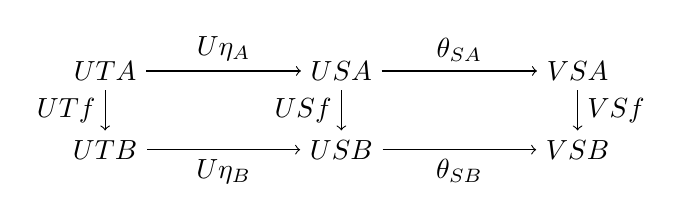
\begin{tikzpicture}
                \node (uta) at (-3,0.5) {\(UTA\)};
                \node (usa) at (0,0.5) {\(USA\)};
                \node (vsa) at (3,0.5) {\(VSA\)};
                \node (utb) at (-3,-0.5) {\(UTB\)};
                \node (usb) at (0,-0.5) {\(USB\)};
                \node (vsb) at (3,-0.5) {\(VSB\)};

                \draw[->] (uta) to node[above] {\(U \eta_A\)} (usa);
                \draw[->] (usa) to node[above] {\(\theta_{SA}\)} (vsa);
                \draw[->] (utb) to node[below] {\(U \eta_B\)} (usb);
                \draw[->] (usb) to node[below] {\(\theta_{SB}\)} (vsb);
                \draw[->] (uta) to node[left] {\(UT f\)} (utb);
                \draw[->] (usa) to node[left] {\(US f\)} (usb);
                \draw[->] (vsa) to node[right] {\(VS f\)} (vsb);
            \end{tikzpicture}
        \end{center}

        我们现在修改这个交换图表, 使得它在 \(\mathfrak{V}\) - 充实范畴中交换,
        对此, 我们将从左上角到右下角的所有路径写出来如下:

        \begin{center}
            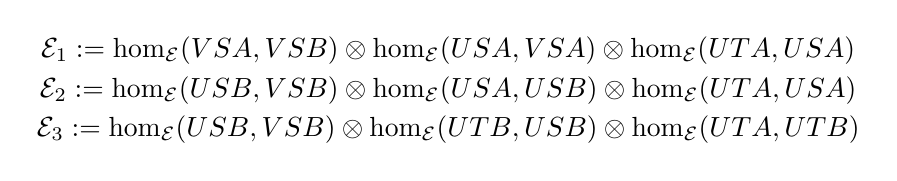
\begin{tikzpicture}
                \node (E1) at (0,0.5) {\(\mathcal{E}_1 := \mathrm{hom}_{\mathcal{E}} (VSA,VSB) \otimes \mathrm{hom}_{\mathcal{E}} (USA,VSA) \otimes \mathrm{hom}_{\mathcal{E}} (UTA,USA)\)};
                \node (E2) at (0,0) {\(\mathcal{E}_2 := \mathrm{hom}_{\mathcal{E}} (USB,VSB) \otimes \mathrm{hom}_{\mathcal{E}} (USA,USB) \otimes \mathrm{hom}_{\mathcal{E}} (UTA,USA)\)};
                \node (E3) at (0,-0.5) {\(\mathcal{E}_3 := \mathrm{hom}_{\mathcal{E}} (USB,VSB) \otimes \mathrm{hom}_{\mathcal{E}} (UTB,USB) \otimes \mathrm{hom}_{\mathcal{E}} (UTA,UTB)\)};
            \end{tikzpicture}
        \end{center}

        由于其中的某些态射是自然变换诱导出的, 确定的, 某些态射是由函子对相同态射给出的, 我们给出不同层级下的路径:

        \begin{center}
            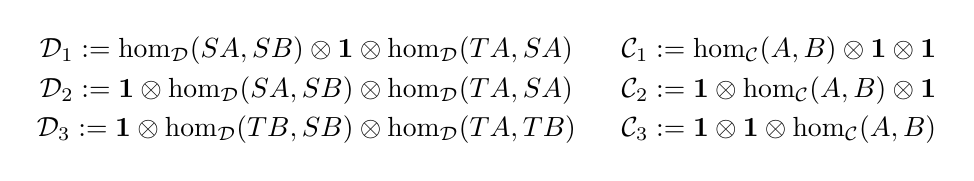
\begin{tikzpicture}
                \node (D1) at (-3,0.5) {\(\mathcal{D}_1 := \mathrm{hom}_{\mathcal{D}} (SA,SB) \otimes \mathbf{1} \otimes \mathrm{hom}_{\mathcal{D}} (TA,SA)\)};
                \node (D2) at (-3,0) {\(\mathcal{D}_2 := \mathbf{1} \otimes \mathrm{hom}_{\mathcal{D}} (SA,SB) \otimes \mathrm{hom}_{\mathcal{D}} (TA,SA)\)};
                \node (D3) at (-3,-0.5) {\(\mathcal{D}_3 := \mathbf{1} \otimes \mathrm{hom}_{\mathcal{D}} (TB,SB) \otimes \mathrm{hom}_{\mathcal{D}} (TA,TB)\)};
                \node (C1) at (3,0.5) {\(\mathcal{C}_1 := \mathrm{hom}_{\mathcal{C}} (A,B) \otimes \mathbf{1} \otimes \mathbf{1}\)};
                \node (C2) at (3,0) {\(\mathcal{C}_2 := \mathbf{1} \otimes \mathrm{hom}_{\mathcal{C}} (A,B) \otimes \mathbf{1}\)};
                \node (C3) at (3,-0.5) {\(\mathcal{C}_3 := \mathbf{1} \otimes \mathbf{1} \otimes \mathrm{hom}_{\mathcal{C}} (A,B)\)};
            \end{tikzpicture}
        \end{center}

        此外, 我们还有条件说明左边正方形和右边正方形的图表分别交换, 同理也拆出对应的态射集合.

        \begin{center}
            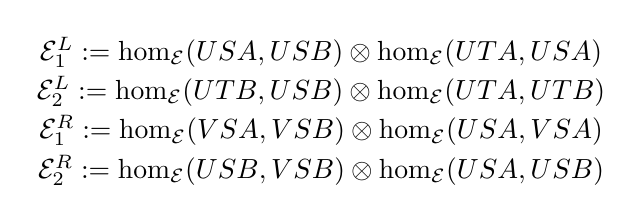
\begin{tikzpicture}
                \node (EL1) at (0,0.75) {\(\mathcal{E}_1^{L} := \mathrm{hom}_{\mathcal{E}} (USA,USB) \otimes \mathrm{hom}_{\mathcal{E}} (UTA,USA)\)};
                \node (EL2) at (0,0.25) {\(\mathcal{E}_2^{L} := \mathrm{hom}_{\mathcal{E}} (UTB,USB) \otimes \mathrm{hom}_{\mathcal{E}} (UTA,UTB)\)};
                \node (ER1) at (0,-0.25) {\(\mathcal{E}_1^{R} := \mathrm{hom}_{\mathcal{E}} (VSA,VSB) \otimes \mathrm{hom}_{\mathcal{E}} (USA,VSA)\)};
                \node (ER2) at (0,-0.75) {\(\mathcal{E}_2^{R} := \mathrm{hom}_{\mathcal{E}} (USB,VSB) \otimes \mathrm{hom}_{\mathcal{E}} (USA,USB)\)};
            \end{tikzpicture}
        \end{center}

        同理, 也写出上述对象在不同层级下的路径:

        \begin{center}
            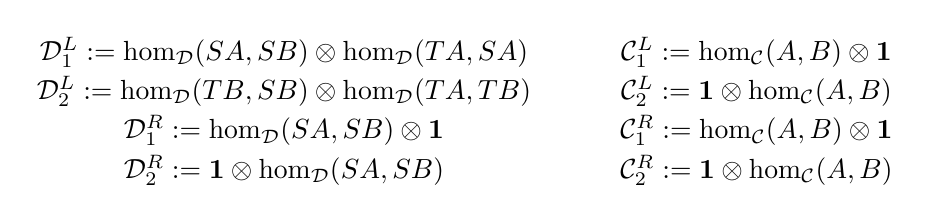
\begin{tikzpicture}
                \node (DL1) at (-3,0.75) {\(\mathcal{D}_1^{L} := \mathrm{hom}_{\mathcal{D}} (SA,SB) \otimes \mathrm{hom}_{\mathcal{D}} (TA,SA)\)};
                \node (DL2) at (-3,0.25) {\(\mathcal{D}_2^{L} := \mathrm{hom}_{\mathcal{D}} (TB,SB) \otimes \mathrm{hom}_{\mathcal{D}} (TA,TB)\)};
                \node (DR1) at (-3,-0.25) {\(\mathcal{D}_1^{R} := \mathrm{hom}_{\mathcal{D}} (SA,SB) \otimes \mathbf{1}\)};
                \node (DR2) at (-3,-0.75) {\(\mathcal{D}_2^{R} := \mathbf{1} \otimes \mathrm{hom}_{\mathcal{D}} (SA,SB)\)};
                \node (CL1) at (3,0.75) {\(\mathcal{C}_1^{L} := \mathrm{hom}_{\mathcal{C}} (A,B) \otimes \mathbf{1}\)};
                \node (CL2) at (3,0.25) {\(\mathcal{C}_2^{L} := \mathbf{1} \otimes \mathrm{hom}_{\mathcal{C}} (A,B)\)};
                \node (CR1) at (3,-0.25) {\(\mathcal{C}_1^{R} := \mathrm{hom}_{\mathcal{C}} (A,B) \otimes \mathbf{1}\)};
                \node (CR2) at (3,-0.75) {\(\mathcal{C}_2^{R} := \mathbf{1} \otimes \mathrm{hom}_{\mathcal{C}} (A,B)\)};
            \end{tikzpicture}
        \end{center}

        利用上述给出的对象重写条件, 我们可以得到以下交换图表:

        \begin{center}
            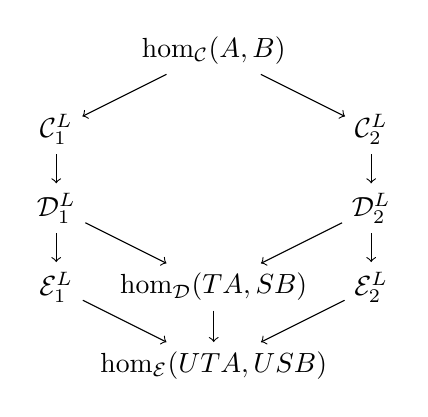
\begin{tikzpicture}
                \node (start) at (0,2) {\(\mathrm{hom}_{\mathcal{C}} (A,B)\)};
                \node (end) at (0,-2) {\(\mathrm{hom}_{\mathcal{E}} (UTA,USB)\)};
                \node (CL1) at (-2,1) {\(\mathcal{C}_1^{L}\)};
                \node (DL1) at (-2,0) {\(\mathcal{D}_1^{L}\)};
                \node (EL1) at (-2,-1) {\(\mathcal{E}_1^{L}\)};
                \node (CL2) at (2,1) {\(\mathcal{C}_2^{L}\)};
                \node (DL2) at (2,0) {\(\mathcal{D}_2^{L}\)};
                \node (EL2) at (2,-1) {\(\mathcal{E}_2^{L}\)};
                \node (middle) at (0,-1) {\(\mathrm{hom}_{\mathcal{D}} (TA,SB)\)};
                
                \draw[->] (start) to (CL1); \draw[->] (CL1) to (DL1); \draw[->] (DL1) to (EL1); \draw[->] (EL1) to (end);
                \draw[->] (start) to (CL2); \draw[->] (CL2) to (DL2); \draw[->] (DL2) to (EL2); \draw[->] (EL2) to (end);
                \draw[->] (DL1) to (middle); \draw[->] (DL2) to (middle); \draw[->] (middle) to (end);
            \end{tikzpicture} 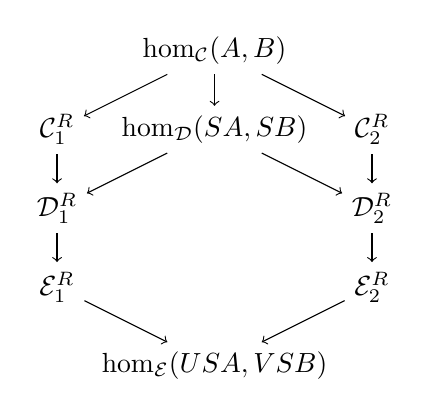
\begin{tikzpicture}
                \node (start) at (0,2) {\(\mathrm{hom}_{\mathcal{C}} (A,B)\)};
                \node (end) at (0,-2) {\(\mathrm{hom}_{\mathcal{E}} (USA,VSB)\)};
                \node (CR1) at (-2,1) {\(\mathcal{C}_1^{R}\)};
                \node (DR1) at (-2,0) {\(\mathcal{D}_1^{R}\)};
                \node (ER1) at (-2,-1) {\(\mathcal{E}_1^{R}\)};
                \node (CR2) at (2,1) {\(\mathcal{C}_2^{R}\)};
                \node (DR2) at (2,0) {\(\mathcal{D}_2^{R}\)};
                \node (ER2) at (2,-1) {\(\mathcal{E}_2^{R}\)};
                \node (middle) at (0,1) {\(\mathrm{hom}_{\mathcal{D}} (SA,SB)\)};

                \draw[->] (start) to (CR1); \draw[->] (CR1) to (DR1); \draw[->] (DR1) to (ER1); \draw[->] (ER1) to (end);
                \draw[->] (start) to (CR2); \draw[->] (CR2) to (DR2); \draw[->] (DR2) to (ER2); \draw[->] (ER2) to (end);
                \draw[->] (start) to (middle); \draw[->] (middle) to (DR1); \draw[->] (middle) to (DR2);
            \end{tikzpicture}
        \end{center}

        上图中对于 \(Sf\) 的给出, 我们在无 \(S\) 的层级中给出对应图表然后再利用 \(S\) 函子性给出上半部分.
        对于 \(U\) 的这步推出, 我们亦在无 \(U\) 的层级中给出对应图表然后再利用 \(U\) 函子性给出下半部分.

        考察到条件图与需求图相差一个 \(\otimes \theta_{SB}\)
        和 \(U \eta_A \otimes\), 在最上方与最下方写一个分离出 \(\otimes\) 的对象, 令
        \(O_1 := \mathrm{hom}_{\mathcal{E}} (USA,VSB) \otimes \mathrm{hom}_{\mathcal{E}} (UTA,USA)\),
        \(O_2 := \mathrm{hom}_{\mathcal{E}} (USB,VSB) \otimes \mathrm{hom}_{\mathcal{E}} (UTA,USB)\),

        \begin{center}
            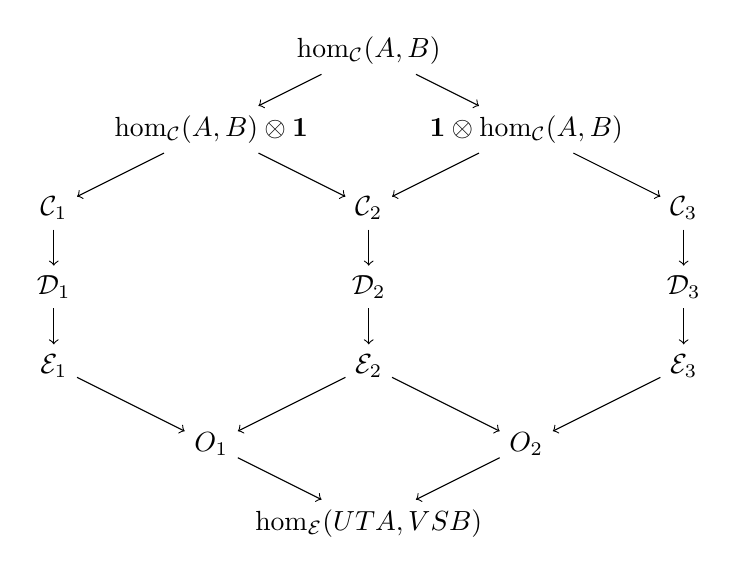
\begin{tikzpicture}
                \node (start) at (0,3) {\(\mathrm{hom}_{\mathcal{C}} (A,B)\)};
                \node (end) at (0,-3) {\(\mathrm{hom}_{\mathcal{E}} (UTA,VSB)\)};
                \node (C1) at (-4,1) {\(\mathcal{C}_1\)};
                \node (C2) at (0,1) {\(\mathcal{C}_2\)};
                \node (C3) at (4,1) {\(\mathcal{C}_3\)};
                \node (D1) at (-4,0) {\(\mathcal{D}_1\)};
                \node (D2) at (0,0) {\(\mathcal{D}_2\)};
                \node (D3) at (4,0) {\(\mathcal{D}_3\)};
                \node (E1) at (-4,-1) {\(\mathcal{E}_1\)};
                \node (E2) at (0,-1) {\(\mathcal{E}_2\)};
                \node (E3) at (4,-1) {\(\mathcal{E}_3\)};
                \node (aboveleft) at (-2,2) {\(\mathrm{hom}_{\mathcal{C}} (A,B) \otimes \mathbf{1}\)};
                \node (aboveright) at (2,2) {\(\mathbf{1} \otimes \mathrm{hom}_{\mathcal{C}} (A,B)\)};
                \node (belowleft) at (-2,-2) {\(O_1\)};
                \node (belowright) at (2,-2) {\(O_2\)};

                \draw[->] (start) to (aboveleft); \draw[->] (aboveleft) to (C1); \draw[->] (C1) to (D1); \draw[->] (D1) to (E1); \draw[->] (E1) to (belowleft); \draw[->] (belowleft) to (end);
                \draw[->] (start) to (aboveright); \draw[->] (aboveright) to (C3); \draw[->] (C3) to (D3); \draw[->] (D3) to (E3); \draw[->] (E3) to (belowright); \draw[->] (belowright) to (end);
                \draw[->] (aboveleft) to (C2); \draw[->] (aboveright) to (C2); \draw[->] (C2) to (D2); \draw[->] (D2) to (E2); \draw[->] (E2) to (belowleft); \draw[->] (E2) to (belowright);
            \end{tikzpicture}
        \end{center}

        此图表交换, 外框给出横合成自然.
    \end{proof}
\end{definition}

\begin{lemma}
    纵合成, 横合成间交换, 纵合成横合成结合.

    \begin{proof}
        仿照上述证明.
    \end{proof}
\end{lemma}

\begin{definition}
    有严格 \(2\) - 范畴 \(\mathfrak{V} - \mathbf{Cat}\).
\end{definition}

\begin{lemma}
    幺半函子 \(F : \mathfrak{V} \to \mathfrak{W}\) 诱导出 \(2\) - 函子 \(F - \mathbf{Cat} : \mathfrak{V} - \mathbf{Cat} \to \mathfrak{W} - \mathbf{Cat}\).

    \begin{proof}
        取 \(\mathfrak{V}\) - 范畴 \(\mathcal{C}\), 定义范畴 \(\mathcal{D} := {F - \mathbf{Cat}} (\mathcal{C})\),
        满足 \(\mathrm{Ob} (\mathcal{D}) = (\mathrm{Ob} (\mathcal{C}))\), \(\mathrm{hom}_{\mathcal{D}} (X,Y) = F(\mathrm{hom}_{\mathcal{C}} (X,Y))\),
        \(M^{\mathcal{D}}_{X,Y,Z} = F(M^{\mathcal{C}}_{X,Y,Z}) \circ J_{\mathrm{hom}_\mathcal{C} (Y,Z),\mathrm{hom}_\mathcal{C} (X,Y)}\)
        给出 \(j_A : \mathbf{1} \to F (\mathrm{hom}_{\mathcal{C}} (A,A))\), 易于验证其是 \(\mathfrak{W}\) - 充实范畴.

        对于 \(\mathfrak{V}\) - 充实函子 \(S\), 我们给出 \(\mathfrak{W}\) - 充实函子 \(T\), \(T\) 在对象集上的限制继承自 \(S\),
        且有 \(T_{A,B} = F(S_{A,B})\).

        对于 \(\mathfrak{V}\) - 自然变换 \(\eta\), 我们给出 \(\mathfrak{W}\) - 自然变换 \(\theta_A := F \eta_A \circ \phi\).

        易于验证上述资料给出 \(\mathfrak{V} - \mathbf{Cat}\) 到 \(\mathfrak{W} - \mathbf{Cat}\) 的 \(2\) - 函子.
    \end{proof}
\end{lemma}

\begin{definition}[单位 \(\mathfrak{V}\) - 充实范畴]
    定义范畴 \(\mathcal{I}_{\mathfrak{V}}\) 为只有一个对象且态射为 \(\mathbf{1}\) 的 \(\mathfrak{V}\) - 充实范畴.
\end{definition}

\begin{definition}
    有 \(2\) - 函子 \((-)_0 := \mathrm{hom}_{\mathfrak{V} - \mathbf{Cat}} (\mathcal{I}_{\mathfrak{V}}, -):\mathfrak{V} - \mathbf{Cat} \to \mathbf{Cat}\),
    其像称为该充实范畴的底层范畴.
\end{definition}

\begin{lemma}
    上述定义的 \({(-)}_0\) 即 \(\mathfrak{V} \to (\mathbf{Set}, \times)\) 的幺半函子诱导出的 \(2\) - 函子.
\end{lemma}

\subsubsection{对称结构}

\begin{definition}[辫结构]
    一个幺半范畴 \(\mathfrak{V}\) 是上的一个辫结构, 是指一个 \(\mathfrak{V} \times \mathfrak{V} \to \mathfrak{V}\) 上的一个自然同构
    \(c_{X,Y} : X \otimes Y \to Y \otimes X\), 使得对于所有对象 \(X,Y,Z\) 满足六边形公理.

    \setlabel {六边形公理}
    \label {axiom:hexagon axiom of braiding monoidal category}
    \begin{center}
        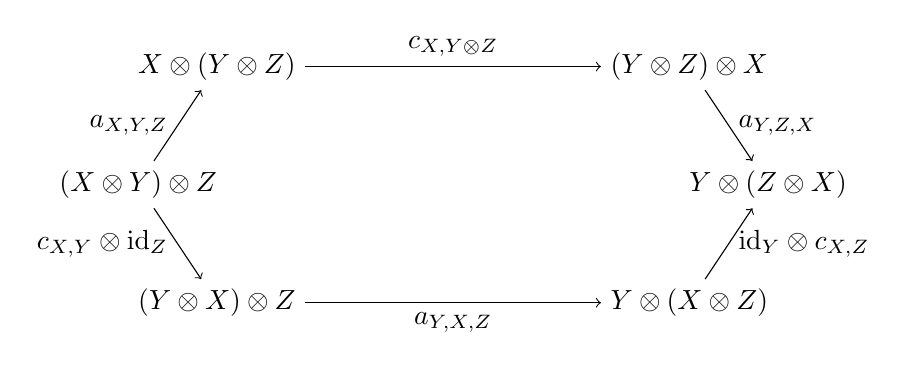
\begin{tikzpicture}
            \node (lxyrz) at (-4,0) {\((X \otimes Y) \otimes Z\)};
            \node (lyxrz) at (-3,-1.5) {\((Y \otimes X) \otimes Z\)};
            \node (ylxzr) at (3,-1.5) {\(Y \otimes (X \otimes Z)\)};
            \node (ylzxr) at (4,0) {\(Y \otimes (Z \otimes X)\)};
            \node (xlyzr) at (-3,1.5) {\(X \otimes (Y \otimes Z)\)};
            \node (lyzrx) at (3,1.5) {\((Y \otimes Z) \otimes X\)};

            \draw[->] (lxyrz) to node[left] {\(c_{X,Y} \otimes \mathrm{id}_Z\)} (lyxrz);
            \draw[->] (lxyrz) to node[left] {\(a_{X,Y,Z}\)} (xlyzr);
            \draw[->] (lyxrz) to node[below] {\(a_{Y,X,Z}\)} (ylxzr);
            \draw[->] (xlyzr) to node[above] {\(c_{X,Y \otimes Z}\)} (lyzrx);
            \draw[->] (ylxzr) to node[right] {\(\mathrm{id}_Y \otimes c_{X,Z}\)} (ylzxr);
            \draw[->] (lyzrx) to node[right] {\(a_{Y,Z,X}\)} (ylzxr);
        \end{tikzpicture}
    \end{center}

    \begin{center}
        \begin{tikzpicture}
            \node (xlyzr) at (-4,0) {\(X \otimes (Y \otimes Z)\)};
            \node (xlzyr) at (-3,-1.5) {\(X \otimes (Z \otimes Y)\)};
            \node (lxzry) at (3,-1.5) {\((X \otimes Z) \otimes Y\)};
            \node (lxyrz) at (-3,1.5) {\((X \otimes Y) \otimes Z\)};
            \node (zlxyr) at (3,1.5) {\(Z \otimes (X \otimes Y)\)};
            \node (lzxry) at (4,0) {\((Z \otimes X) \otimes Y\)};

            \draw[->] (xlyzr) to node[left] {\(\mathrm{id}_X \otimes c_{Y,Z}\)} (xlzyr);
            \draw[->] (xlyzr) to node[left] {\(a^{-1}_{X,Y,Z}\)} (lxyrz);
            \draw[->] (xlzyr) to node[below] {\(a^{-1}_{X,Z,Y}\)} (lxzry);
            \draw[->] (lxyrz) to node[above] {\(c_{X \otimes Y,Z}\)} (zlxyr);
            \draw[->] (lxzry) to node[right] {\(c_{X,Z} \otimes \mathrm{id}_Y\)} (lzxry);
            \draw[->] (zlxyr) to node[right] {\(a^{-1}_{Z,X,Y}\)} (lzxry);
        \end{tikzpicture}
    \end{center}
\end{definition}

\begin{definition}
    一个辫幺半范畴是一个带辫结构的幺半范畴.
\end{definition}

\begin{definition}
    辫幺半范畴 \(\mathfrak{V}\) 若使 \(c^\prime_{X,Y} = c^{-1}_{Y,X}\) 也构成辫幺半范畴, 记作 \(\mathfrak{V}^{rev}\).
\end{definition}

\begin{lemma}
    有交换图表:

    \begin{center}
        \begin{tikzpicture}
            \node (x) at (-1.5,0) {\(X\)};
            \node (x1) at (1,1) {\(X \otimes \mathbf{1}\)};
            \node (1x) at (1,-1) {\(\mathbf{1} \otimes X\)};

            \draw[->] (x1) to node[above] {\(\rho_X\)} (x);
            \draw[->] (1x) to node[below] {\(\lambda_X\)} (x);
            \draw[->] (x1) to node[right] {\(c_{X,\mathbf{1}}\)} (1x);
        \end{tikzpicture} \begin{tikzpicture}
            \node (x) at (1.5,0) {\(X\)};
            \node (x1) at (-1,1) {\(\mathbf{1} \otimes X\)};
            \node (1x) at (-1,-1) {\(X \otimes \mathbf{1}\)};

            \draw[->] (x1) to node[above] {\(\lambda_X\)} (x);
            \draw[->] (1x) to node[below] {\(\rho_X\)} (x);
            \draw[->] (x1) to node[left] {\(c_{\mathbf{1},X}\)} (1x);
        \end{tikzpicture}
    \end{center}

    \begin{proof}
        外框和其他小图形交换, 故最下方小三角形交换.

        \begin{center}
            \begin{tikzpicture}
                \node (11 x) at (-4,2) {\((\mathbf{1} \otimes \mathbf{1}) \otimes X\)};
                \node (1 1x) at (4,2) {\(\mathbf{1} \otimes (\mathbf{1} \otimes X)\)};
                \node (x 11) at (-4,0) {\(X \otimes (\mathbf{1} \otimes \mathbf{1})\)};
                \node (1 x1) at (4,0) {\(\mathbf{1} \otimes (X \otimes \mathbf{1})\)};
                \node (x1 1) at (-4,-2) {\((X \otimes \mathbf{1}) \otimes \mathbf{1}\)};
                \node (1x 1) at (4,-2) {\((\mathbf{1} \otimes X) \otimes \mathbf{1}\)};
                \node (1x) at (0,1) {\(\mathbf{1} \otimes X\)};
                \node (x1) at (0,-1) {\(X \otimes \mathbf{1}\)};

                \draw[->] (x1 1) to node[left] {\(a_{X,\mathbf{1},\mathbf{1}}\)} (x 11);
                \draw[->] (x 11) to node[left] {\(c_{X,\mathbf{1} \otimes \mathbf{1}}\)} (11 x);
                \draw[->] (11 x) to node[above] {\(a_{\mathbf{1},\mathbf{1},X}\)} (1 1x);
                \draw[->] (x1 1) to node[below] {\(c_{X,\mathbf{1}} \otimes \mathrm{id}_{\mathbf{1}}\)} (1x 1);
                \draw[->] (1x 1) to node[right] {\(a_{\mathbf{1},X,\mathbf{1}}\)} (1 x1);
                \draw[->] (1 x1) to node[right] {\(\mathrm{id}_{\mathbf{1}} \otimes c_{X,\mathbf{1}}\)} (1 1x);
                \draw[->] (11 x) to node {\(\iota \otimes \mathrm{id}_X\)} (1x);
                \draw[->] (1 1x) to node {\(\lambda_{\mathbf{1} \otimes X} = \mathrm{id}_{\mathbf{1}} \otimes \lambda_X\)} (1x);
                \draw[->] (x 11) to node {\(\mathrm{id}_X \otimes \iota\)} (x1);
                \draw[->] (1 x1) to node {\(\lambda_{X \otimes \mathbf{1}}\)} (x1);
                \draw[->] (x1 1) to node {\(\rho_X \otimes \mathrm{id}_{\mathbf{1}} = \rho_{X \otimes \mathrm{id}_{\mathbf{1}}}\)} (x1);
                \draw[->] (1x 1) to node {\(\lambda_X \otimes \mathrm{id}_{\mathbf{1}}\)} (x1);
                \draw[->] (x1) to node {\(c_{X,\mathbf{1}}\)} (1x);
            \end{tikzpicture}
        \end{center}

        在 \(\mathfrak{V}^{rev}\) 中考虑, 即得另一个方向的交换图表.
    \end{proof}
\end{lemma}

\begin{lemma}[Yang-Baxter]
    略去结合约束, 辫结构 \(c\) 满足 Yang-Baxter 方程如下:

    \[
        (c_{Y,Z} \otimes \mathrm{id}_X) \circ (\mathrm{id}_Y \otimes c_{X,Z}) \circ (c_{X,Y} \otimes \mathrm{id}_Z) = 
        (\mathrm{id}_Z \otimes c_{X,Y}) \circ (c_{X,Z} \otimes \mathrm{id}_Y) \circ (\mathrm{id}_X \otimes c_{Y,Z})
    \]

    \begin{proof}
        有以下交换图表, 左右两边源自 \ref{axiom:hexagon axiom of braiding monoidal category}, 中间源自 \(c\) 自然性:

        \begin{center}
            \begin{tikzpicture}
                \node (xy z) at (-4.5,1.5) {\((X \otimes Y) \otimes Z\)};
                \node (x yz) at (-1.5,1.5) {\(X \otimes (Y \otimes Z)\)};
                \node (x zy) at (1.5,1.5) {\(X \otimes (Z \otimes Y)\)};
                \node (xz y) at (4.5,1.5) {\((X \otimes Z) \otimes Y\)};
                \node (zx y) at (4.5,0.5) {\((Z \otimes X) \otimes Y\)};
                \node (z xy) at (4.5,-0.5) {\(Z \otimes (X \otimes Y)\)};
                \node (z yx) at (4.5,-1.5) {\(Z \otimes (Y \otimes X)\)};
                \node (zy x) at (1.5,-1.5) {\((Z \otimes Y) \otimes X\)};
                \node (yz x) at (-1.5,-1.5) {\((Y \otimes Z) \otimes X\)};
                \node (y zx) at (-4.5,-1.5) {\(Y \otimes (Z \otimes X)\)};
                \node (y xz) at (-4.5,-0.5) {\(Y \otimes (X \otimes Z)\)};
                \node (yx z) at (-4.5,0.5) {\((Y \otimes X) \otimes Z\)};

                \draw[->] (xy z) to node[above] {\(a_{X,Y,Z}\)} (x yz); \draw[->] (x yz) to node[above] {\(\mathrm{id}_X \otimes c_{Y,Z}\)} (x zy); \draw[->] (x zy) to node[above] {\(a^{-1}_{X,Z,Y}\)} (xz y);
                \draw[->] (xz y) to node[right] {\(c_{X,Z} \otimes \mathrm{id}_Y\)} (zx y); \draw[->] (zx y) to node[right] {\(a_{Z,X,Y}\)} (z xy); \draw[->] (z xy) to node[right] {\(\mathrm{id}_Z \otimes c_{X,Y}\)} (z yx);
                \draw[->] (xy z) to node[right] {\(c_{X,Y} \otimes \mathrm{id}_Z\)} (yx z); \draw[->] (yx z) to node[right] {\(a_{Y,X,Z}\)} (y xz); \draw[->] (y xz) to node[right] {\(\mathrm{id}_Y \otimes c_{X,Z}\)} (y zx);
                \draw[->] (y zx) to node[below] {\(a^{-1}_{Y,Z,X}\)} (yz x); \draw[->] (yz x) to node[below] {\(c_{Y,Z} \otimes \mathrm{id}_X\)} (zy x); \draw[->] (zy x) to node[below] {\(a_{Z,Y,X}\)} (z yx);
                \draw[dashed,->] (x yz) to node[right] {\(c_{X,Y \otimes Z}\)} (yz x);
                \draw[dashed,->] (x zy) to node[right] {\(c_{X,Z \otimes Y}\)} (zy x);
            \end{tikzpicture}
        \end{center}
    \end{proof}
\end{lemma}

\begin{remark}
    使用辫图的语言, 我们可以改写上述方程, \(c\) 的自然性意味着:

    \begin{center}
        \begin{tikzpicture}
            \pic[
                braid/number of strands=2,
                ultra thick,
                braid/strand 1/.style={red},
                braid/strand 2/.style={blue},
                braid/gap=0.1,
                braid/border height=15pt,
            ] (left) at (-2,0) {braid={s_1}};
            \node[circle,draw,fill=white,inner sep=0pt,outer sep=0pt,minimum size = 18pt] at (left-1-1) {\(f\)};
            \node[circle,draw,fill=white,inner sep=0pt,outer sep=0pt,minimum size = 18pt] at (left-2-1) {\(g\)};

            \pic[
                braid/number of strands=2,
                ultra thick,
                braid/strand 1/.style={red},
                braid/strand 2/.style={blue},
                braid/gap=0.1,
                braid/border height=15pt,
            ] (right) at (2,0) {braid={s_1}};
            \node[circle,draw,fill=white,inner sep=0pt,outer sep=0pt,minimum size = 18pt] at (right-1-0) {\(f\)};
            \node[circle,draw,fill=white,inner sep=0pt,outer sep=0pt,minimum size = 18pt] at (right-2-0) {\(g\)};

            \node at ($(left.center)!.5!(right.center)$) {\(=\)};
        \end{tikzpicture}
    \end{center}

    \ref{axiom:hexagon axiom of braiding monoidal category} 意味着可以把两条相邻的线绑定.

    此时 Yang-Baxter 方程可以改写为辫图的等价:

    \begin{center}
        \begin{tikzpicture}
            \pic[
                braid/number of strands=3,
                ultra thick,
                braid/strand 1/.style={red},
                braid/strand 2/.style={blue},
                braid/strand 3/.style={black},
                braid/gap=0.1,
                braid/border height=15pt,
            ] (left) at (-2,0) {braid={s_{1,2} s_{2,3} s_{1,2}}};

            \pic[
                braid/number of strands=3,
                ultra thick,
                braid/strand 1/.style={red},
                braid/strand 2/.style={blue},
                braid/strand 3/.style={black},
                braid/gap=0.1,
                braid/border height=15pt,
            ] (right) at (2,0) {braid={s_{2,3} s_{1,2} s_{2,3}}};

            \node at ($(left.center)!.5!(right.center)$) {\(=\)};
        \end{tikzpicture}
    \end{center}

    证明过程无非是把蓝线和黑线绑定, 运用 \(c\) 的自然性将左下角的交叉挪到右上角,
    再将蓝线和黑线解绑拆开.
\end{remark}

\begin{definition}
    一个对称结构是在辫结构的基础上额外要求 \(c_{X,Y} \circ c_{Y,X} = \mathrm{id}_{Y \otimes X}\) 的辫 \(c\),
    带有对称结构的幺半范畴称对称幺半范畴.
\end{definition}

\begin{definition}
    在对称幺半范畴 \(\mathfrak{V}\) 上可以定义两 \(\mathfrak{V}\) - 充实范畴 \(\mathcal{A}, \mathcal{B}\) 的张量积 \(\mathcal{A} \otimes \mathcal{B}\),
    其对象集 \(\mathrm{Ob} (\mathcal{A} \otimes \mathcal{B}) = \mathrm{Ob} (\mathcal{A}) \times \mathrm{Ob} (\mathcal{B})\), 定义态射
    \(\mathrm{hom}_{\mathcal{A} \otimes \mathcal{B}} ((A,B),(A^\prime,B^\prime)) := \mathrm{hom}_{\mathcal{A}} (A,A^\prime) \otimes \mathrm{hom}_{\mathcal{B}} (B,B^\prime)\),
    态射的合成和单位态射定义如下:

    \begin{center}
        \begin{tikzpicture}
            \node (o) at (0,1) {\((\mathrm{hom}_{\mathcal{A}} (A^\prime,A^{\prime \prime}) \otimes \mathrm{hom}_{\mathcal{B}} (B^\prime,B^{\prime \prime})) \otimes (\mathrm{hom}_{\mathcal{A}} (A,A^{\prime}) \otimes \mathrm{hom}_{\mathcal{B}} (B,B^{\prime}))\)};
            \node (c) at (0,0) {\((\mathrm{hom}_{\mathcal{A}} (A^\prime,A^{\prime \prime}) \otimes \mathrm{hom}_{\mathcal{A}} (A,A^{\prime})) \otimes (\mathrm{hom}_{\mathcal{B}} (B^\prime,B^{\prime \prime}) \otimes \mathrm{hom}_{\mathcal{B}} (B,B^{\prime}))\)};
            \node (r) at (0,-1) {\(\mathrm{hom}_{\mathcal{A}} (A,A^{\prime \prime}) \otimes \mathrm{hom}_{\mathcal{B}} (B^\prime,B^{\prime \prime})\)};

            \draw[->] (o) to (c);
            \draw[->] (c) to node[left] {\(M^{\mathcal{A}}_{A,A^\prime,A^{\prime \prime}} \otimes M^{\mathcal{B}}_{B,B^\prime,B^{\prime \prime}}\)} (r);
        \end{tikzpicture}

        \begin{tikzpicture}
            \node (i) at (-3,0) {\(\mathbf{1}\)};
            \node (ii) at (-1.5,0) {\(\mathbf{1} \otimes \mathbf{1}\)};
            \node (hahb) at (3,0) {\(\mathrm{hom}_{\mathcal{A}} (A,A) \otimes \mathrm{hom}_{\mathcal{B}} (B,B)\)};

            \draw[->] (i) to node[above] {\(\iota^{-1}\)} (ii);
            \draw[->] (ii) to node[above] {\(j^\mathcal{A}_A \otimes j^\mathcal{B}_B\)} (hahb);
        \end{tikzpicture}
    \end{center}

    \begin{proof}
        \(c\) 自然性, 有交换图表:
        
        \[
            \begin{aligned}
                &\mathfrak{A}^{\prime \prime} = \mathrm{hom}_{\mathcal{A}} (A^{\prime \prime},A^{\prime \prime \prime}),
                &\mathfrak{A}^{\prime} = \mathrm{hom}_{\mathcal{A}} (A^{\prime},A^{\prime \prime}), &\mathfrak{A} = \mathrm{hom}_{\mathcal{A}} (A,A^{\prime}) \\
                &\mathfrak{B}^{\prime \prime} = \mathrm{hom}_{\mathcal{B}} (B^{\prime \prime},B^{\prime \prime \prime}),
                &\mathfrak{B}^{\prime} = \mathrm{hom}_{\mathcal{B}} (B^{\prime},B^{\prime \prime}), &\mathfrak{B} = \mathrm{hom}_{\mathcal{B}} (B,B^{\prime})
            \end{aligned}
        \]

        \begin{center}
            \begin{tikzpicture}
                \node (AABBAB) at (-3.3,2) {\(\mathfrak{A}^{\prime \prime} \otimes \mathfrak{A}^{\prime} \otimes \mathfrak{B}^{\prime \prime} \otimes \mathfrak{B}^{\prime} \otimes \mathfrak{A} \otimes \mathfrak{B}\)};
                \node (AAABBB) at (-3.3,0) {\(\mathfrak{A}^{\prime \prime} \otimes \mathfrak{A}^{\prime} \otimes \mathfrak{A} \otimes \mathfrak{B}^{\prime \prime} \otimes \mathfrak{B}^{\prime} \otimes \mathfrak{B}\)};
                \node (ABAABB) at (-3.3,-2) {\(\mathfrak{A}^{\prime \prime} \otimes \mathfrak{B}^{\prime \prime} \otimes \mathfrak{A}^{\prime} \otimes \mathfrak{A} \otimes \mathfrak{B}^{\prime} \otimes \mathfrak{B}\)};
                \node (ABAB1) at (3.3,2) {\(\mathrm{hom}_{\mathcal{A}} (A^\prime,A^{\prime \prime \prime}) \otimes \mathrm{hom}_{\mathcal{B}} (B^\prime,B^{\prime \prime \prime}) \otimes \mathfrak{A} \otimes \mathfrak{B}\)};
                \node (AABB1) at (3.3,1) {\(\mathrm{hom}_{\mathcal{A}} (A^\prime,A^{\prime \prime \prime}) \otimes \mathfrak{A} \otimes \mathrm{hom}_{\mathcal{B}} (B^\prime,B^{\prime \prime \prime}) \otimes \mathfrak{B}\)};
                \node (AABB2) at (3.3,-1) {\(\mathfrak{A}^{\prime \prime} \otimes \mathrm{hom}_{\mathcal{A}} (A,A^{\prime \prime}) \otimes \mathfrak{B}^{\prime \prime} \otimes \mathrm{hom}_{\mathcal{B}} (B,B^{\prime \prime})\)};
                \node (ABAB2) at (3.3,-2) {\(\mathfrak{A}^{\prime \prime} \otimes \mathfrak{B}^{\prime \prime} \otimes \mathrm{hom}_{\mathcal{A}} (A,A^{\prime \prime}) \otimes \mathrm{hom}_{\mathcal{B}} (B,B^{\prime \prime})\)};
                \node (AB) at (3.3,0) {\(\mathrm{hom}_{\mathcal{A}} (A,A^{\prime \prime \prime}) \otimes \mathrm{hom}_{\mathcal{B}} (B,B^{\prime \prime \prime})\)};

                \draw[->] (AABBAB) to (ABAB1); \draw[->] (ABAABB) to (ABAB2);
                \draw[->] (AAABBB) to (AABB1); \draw[->] (AAABBB) to (AABB2);
                \draw[->] (AABBAB) to (AAABBB); \draw[->] (ABAABB) to (AAABBB);
                \draw[->] (ABAB1) to (AABB1); \draw[->] (ABAB2) to (AABB2); \draw[->] (AABB1) to (AB); \draw[->] (AABB2) to (AB);
            \end{tikzpicture}
        \end{center}

        同理, 单位映射需注意到交换图表:

        \begin{center}
            \begin{tikzpicture}
                \node (11AB) at (-3.2,0.5) {\(\mathbf{1} \otimes \mathbf{1} \otimes \mathfrak{A} \otimes \mathfrak{B}\)};
                \node (1A1B) at (3.2,0.5) {\(\mathbf{1} \otimes \mathfrak{A} \otimes \mathbf{1} \otimes \mathfrak{B}\)};
                \node (hhAB) at (-3.2,-0.5) {\(\mathrm{hom}_{\mathcal{A}} (A,A) \otimes \mathrm{hom}_{\mathcal{B}} (B,B) \otimes \mathfrak{A} \otimes \mathfrak{B}\)};
                \node (hAhB) at (3.2,-0.5) {\(\mathrm{hom}_{\mathcal{A}} (A,A) \otimes \mathfrak{A} \otimes \mathrm{hom}_{\mathcal{B}} (B,B) \otimes \mathfrak{B}\)};

                \draw[->] (11AB) to (1A1B); \draw[->] (hhAB) to (hAhB);
                \draw[->] (11AB) to node[left] {\(j^\mathcal{A}_A \otimes j^\mathcal{B}_B\)} (hhAB); \draw[->] (1A1B) to node[right] {\(j^\mathcal{A}_A \otimes j^\mathcal{B}_B\)} (hAhB);
            \end{tikzpicture}
        \end{center}
    \end{proof}
\end{definition}

\begin{definition}
    在对称幺半范畴 \(\mathfrak{V}\) 上可以定义一个 \(\mathfrak{V}\) - 充实范畴 \(\mathcal{A}\) 的对偶范畴 \(\mathcal{A}^{\mathrm{op}}\),,
    其对象为 \(\mathrm{Ob} (\mathcal{A}^{\mathrm{op}}) := \mathrm{Ob} (\mathcal{A})\), 定义态射 \(\mathrm{hom}_{\mathcal{A}^{\mathrm{op}}} (A,B) := \mathrm{hom}_{\mathcal{A}} (B,A)\),
    单位态射定义不变, 态射的合成定义如下:

    \begin{center}
        \begin{tikzpicture}
            \node (o) at (0,1) {\(\mathrm{hom}_{\mathcal{A}} (A,B) \otimes \mathrm{hom}_{\mathcal{A}} (B,C)\)};
            \node (c) at (0,0) {\(\mathrm{hom}_{\mathcal{A}} (B,C) \otimes \mathrm{hom}_{\mathcal{A}} (A,B)\)};
            \node (r) at (0,-1) {\(\mathrm{hom}_{\mathcal{A}} (A,C)\)};

            \draw[->] (o) to (c);
            \draw[->] (c) to node[left] {\(M^{\mathcal{A}}_{A,B,C}\)} (r);
        \end{tikzpicture}
    \end{center}
\end{definition}

\begin{lemma}
    对称幺半范畴若有内 \(\mathrm{Hom}\) 对象则 \ref{definition:biclosed monoidal category},
    且 \([\![X,Y]\!]\) 有典范的选取 \([\![X,Y]\!] = [X,Y]\).
\end{lemma}

\begin{remark}
    我们也记内 \(Hom\) 对象为 \([X,Y]\), 也记\([\![X,Y]\!]\), 同构写作 
    \(\varphi : \mathrm{Hom} (X \otimes Y,Z) \to \mathrm{Hom} (X,[Y,Z])\),
    \(\psi : \mathrm{Hom} (X \otimes Y,Z) \to \mathrm{Hom} (Y,[\![X,Z]\!])\).
\end{remark}

\begin{remark}
    利用 \ref{definition:internal hom canonical functor} 可以给出内 \(\mathrm{Hom}\) 对象的复合,
    而利用 \(\varphi (\lambda_X)\) 可以给出单位态射, 从而 \ref{definition:biclosed monoidal category} 的 \(\mathfrak{V}\) 是 \(\mathfrak{V}\) - 充实范畴.
\end{remark}

\begin{definition}
    若 \(\mathfrak{V}\) 是对称幺半范畴, 则 \(\mathfrak{V}\) - 充实范畴 \(\mathcal{A}\) 有函子 \(\mathrm{hom}_{\mathcal{A}} (-,-) : \mathcal{A}^{\mathrm{op}} \otimes \mathcal{A} \to \mathfrak{V}\),
    其映 \((A,B) \mapsto \mathrm{hom}_{\mathcal{A}} (A,B)\), 需建立态射对象上的态射.

    首先考察结合态射 \(M_{A,B,C} : \mathrm{hom}_{\mathcal{A}} (B,C) \otimes \mathrm{hom}_{\mathcal{A}} (A,B) \to \mathrm{hom}_{\mathcal{A}} (A,C)\), 给出了
    \(\varphi(M_{A,B,C}) : \mathrm{hom}_{\mathcal{A}} (B,C) \to [\mathrm{hom}_{\mathcal{A}} (A,B),\mathrm{hom}_{\mathcal{A}} (A,C)]\), 亦给出
    \(\varphi(M_{A,B,C} \circ c_{\mathrm{hom}_{\mathcal{A}} (B,C),\mathrm{hom}_{\mathcal{A}} (A,B)}) : \mathrm{hom}_{\mathcal{A}} (A,B) \to [\mathrm{hom}_{\mathcal{A}} (B,C),\mathrm{hom}_{\mathcal{A}} (A,C)]\).

    于是给出一个态射对象 \(\mathrm{hom}_{\mathcal{A}} (A^\prime,A) \otimes \mathrm{hom}_{\mathcal{B}} (B,B^\prime)\), 透过上述两类态射给出态射:
    \(\varphi(M_{A^\prime,A,B^\prime} \circ c_{\mathrm{hom}_{\mathcal{A}} (A,B^\prime),\mathrm{hom}_{\mathcal{A}} (A^\prime,A)}) \otimes \varphi(M_{A,B,B^\prime}) : \mathrm{hom}_{\mathcal{A}} (A^\prime,A) \otimes \mathrm{hom}_{\mathcal{B}} (B,B^\prime) \to [\mathrm{hom}_{\mathcal{A}} (A,B^\prime),\mathrm{hom}_{\mathcal{A}} (A^\prime,B^\prime)] \otimes [\mathrm{hom}_{\mathcal{A}} (A,B),\mathrm{hom}_{\mathcal{A}} (A,B^\prime)]\),
    再经典范的合成得到 \(\mathrm{hom}_{\mathcal{A}} (A^\prime,A) \otimes \mathrm{hom}_{\mathcal{B}} (B,B^\prime) \to [\mathrm{hom}_{\mathcal{A}} (A,B), \mathrm{hom}_{\mathcal{A}} (A^\prime,B^\prime)]\).
\end{definition}

\newpage
